% qual o tempo da apresentação? apresento os apêndices? apresento os trabalhos relacionados? apresento as referências (90)?  
%	Name			:: 	sthlm Beamer Theme  HEAVILY based on the hsrmbeamer theme (Benjamin Weiss)
%	Author			:: 	Mark Hendry Olson (mark@hendryolson.com)
%	Created			::	2013-07-31
%	Updated	    	::	[[April]] 04, 2017 at 16:26:39
%	Version			:: 	2.0.2
%	Email			:: 	hendryolson@gmail.com
%	Website			:: 	http://markolson.se
%	Twitter			:: 	markolsonse
%	Instagram		:: 	markolsonse
%
%	License			:: 	This file may be distributed and/or modified under the
%					GNU Public License.
%
%	Description		::	This presentation is a demonstration of the sthlm beamer
%					theme, which is HEAVILY based on the HSRM beamer theme created by Benjamin Weiss
%					(benjamin.weiss@student.hs-rm.de), which can be found on GitHub
%					<https://github.com/hsrmbeamertheme/hsrmbeamertheme>.  It also borrows heavily
%					from the work of Matthias Vogelgesang, (https://bloerg.net) and his Metropolis Mtheme,
%					<https://github.com/matze/mtheme>.
%
%	Theme			::	newPxFont
%	Options			::	progressbar
%					::	sectionpages
%					::	numfooter
%					::	fullfooter
%					::	dovaligncolumns
%					::	protectframetitle
%					::	greybg
%					::	cblock
%					::	minimal

%-=-=-=-=-=-=-=-=-=-=-=-=-=-=-=-=-=-=-=-=-=-=-=-=
%
%        LOADING DOCUMENT
%
%-=-=-=-=-=-=-=-=-=-=-=-=-=-=-=-=-=-=-=-=-=-=-=-=

\documentclass[newPxFont, numfooter, sectionpages]{beamer}
\usepackage[utf8]{inputenc}
\usetheme{sthlm}
\usepackage{pgfplots}
\pgfplotsset{compat=1.9}
\usepackage{cancel}
\usepackage{amsthm,amsmath}
\usepackage{mathtools}

\usepackage{booktabs}
\usepackage{supertabular}
\usepackage{tabularx}
\usepackage{longtable}
\usepackage{multirow}
\usepackage{hhline}
\usepackage{color, colortbl}

\usepackage[backend=bibtex, style=numeric, defernumbers=true]{biblatex}
\addbibresource{../references.bib}

\DeclarePairedDelimiter\abs{\lvert}{\rvert}%
\DeclarePairedDelimiter\norm{\lVert}{\rVert}%

\definecolor{lightgray}{gray}{0.8}
\definecolor{Gray}{gray}{0.9}

\title{Discriminative Sensing Based on Signal Processing for Information Security Analysis}
\subtitle{\small{Ph.D. Thesis Qualification}}
\author{\texttt{Thiago P. de B. Vieira \newline \textbf{Advisor:} João Paulo C. L. da Costa} }
\institute{
		\scriptsize{Universidade de Brasília}
	\\ 	\scriptsize{Departamento de Engenharia Elétrica - ENE/FT}
	\\ \scriptsize{Progama de Pós-Graduação em Engenharia Elétrica - PPGEE}}


\begin{document}

%-=-=-=-=-=-=-=-=-=-=-=-=-=-=-=-=-=-=-=-=-=-=-=-=
%
%	TITLE PAGE
%
%-=-=-=-=-=-=-=-=-=-=-=-=-=-=-=-=-=-=-=-=-=-=-=-=
\maketitle
%-=-=-=-=-=-=-=-=-=-=-=-=-=-=-=-=-=-=-=-=-=-=-=-=
%	FRAME: Theme Package Requirements
%-=-=-=-=-=-=-=-=-=-=-=-=-=-=-=-=-=-=-=-=-=-=-=-=
\begingroup
\setbeamercolor{normal text}{fg=\cnDarkGrey,bg=white}


%-=-=-=-=-=-=-=-=-=-=-=-=-=-=-=-=-=-=-=-=-=-=-=-=
%
%	TABLE OF CONTENTS: OVERVIEW
%
%-=-=-=-=-=-=-=-=-=-=-=-=-=-=-=-=-=-=-=-=-=-=-=-=
\section*{Outline}
\begin{frame}{Outline}
	\tableofcontents[hideallsubsections]% For longer presentations use hideallsubsections option
\end{frame}

%-=-=-=-=-=-=-=-=-=-=-=-=-=-=-=-=-=-=-=-=-=-=-=-=
%
%	TABLE OF CONTENTS: OVERVIEW
%
%-=-=-=-=-=-=-=-=-=-=-=-=-=-=-=-=-=-=-=-=-=-=-=-=
\section{Introduction}
%-=-=-=-=-=-=-=-=-=-=-=-=-=-=-=-=-=-=-=-=-=-=-=-=
%	FRAME: Motivation
%-=-=-=-=-=-=-=-=-=-=-=-=-=-=-=-=-=-=-=-=-=-=-=-=
\begin{frame}[c]{Motivation}
	\begin{itemize}
		\item It is necessary investments to detect \textbf{novel attacks and their variations};
		\item Secure mobile cloud architecture is challenging, specially in \textbf{offline mode}
		\item \textbf{Fraud detection} of \textbf{Mobile Money Transactions} has been motivating investments
		\begin{itemize}
			\item The \textbf{extraction of relevant information} from \textbf{raw or big data} is useful for classification problems and for security analysis.;
			\item \textbf{Imbalanced data is challenging} for classification related to anomaly detection, novelty detection, fraud detection and attack detection.
		\end{itemize}
	\end{itemize}
\end{frame}
%-=-=-=-=-=-=-=-=-=-=-=-=-=-=-=-=-=-=-=-=-=-=-=-=
%	FRAME: Problem Statement
%-=-=-=-=-=-=-=-=-=-=-=-=-=-=-=-=-=-=-=-=-=-=-=-=
\begin{frame}[c]{Problem Statement}
	\textbf{This thesis} outlines the \textbf{development} and evaluation of approaches based on \textbf{signal processing for information security analysis}...
	\begin{itemize}
		\item To make the data \textbf{discriminative for network attack detection, mobile malicious behavior analysis and fraud detection.}
	\end{itemize}
\end{frame}
% %-=-=-=-=-=-=-=-=-=-=-=-=-=-=-=-=-=-=-=-=-=-=-=-=
% %	FRAME: Problem Statement
% %-=-=-=-=-=-=-=-=-=-=-=-=-=-=-=-=-=-=-=-=-=-=-=-=
% \begin{frame}[c]{Problem Statement}
% 	We propose an approach for \textbf{identification of malicious traffic in computer networks}
% 	\begin{itemize}
% 		\item We use\textbf{largest eigenvalues and MOS} to \textbf{network attack detection};
% 		\item We propose \textbf{Eigen similarity analysis} identify \textbf{accurate time and ports} under attack;
% 	\end{itemize}
% \end{frame}
% %-=-=-=-=-=-=-=-=-=-=-=-=-=-=-=-=-=-=-=-=-=-=-=-=
% %	FRAME: Problem Statement
% %-=-=-=-=-=-=-=-=-=-=-=-=-=-=-=-=-=-=-=-=-=-=-=-=
% \begin{frame}[c]{Problem Statement}
% 	This thesis also proposes an \textbf{approach for malicious behavior detection in mobile apps}
% 	\begin{itemize}
% 		\item An \textbf{architecture} for mobile security analysis;
% 		\item \textbf{Offline user behavior analysis} based on MOS;
% 		\item Scenario analysis for \textbf{feature selection};
% 		\item \textbf{Processing time} evaluation in \textbf{mobile} devices.
% 	\end{itemize}
% \end{frame}
% %-=-=-=-=-=-=-=-=-=-=-=-=-=-=-=-=-=-=-=-=-=-=-=-=
% %	FRAME: Problem Statement
% %-=-=-=-=-=-=-=-=-=-=-=-=-=-=-=-=-=-=-=-=-=-=-=-=
% \begin{frame}[c]{Problem Statement}
% 	We finally propose a \textbf{tensor-based dictionary learning method for fraud detection} 
% 	\begin{itemize}
% 		\item Sparse representation based \textbf{classification} (SRC) through learning a \textbf{tensor-based} dictionary;
% 		\item Apply the \textbf{learned dictionaries to reconstruct} a test signal;
% 		\item \textbf{Fraud classification} of mobile money transactions according to the \textbf{reconstruction error}.
% 	\end{itemize}
% \end{frame}
%-=-=-=-=-=-=-=-=-=-=-=-=-=-=-=-=-=-=-=-=-=-=-=-=
%	FRAME: Contributions
%-=-=-=-=-=-=-=-=-=-=-=-=-=-=-=-=-=-=-=-=-=-=-=-=
% \begin{frame}{Contributions}
% 	\begin{enumerate}
% 		\item An approach based on \textbf{eigen similarity analysis} for extracting detailed information about accurate time and network ports under network attack;
% 		\item Computational \textbf{complexity analysis} of the proposed framework;
% 		\item An architecture and techniques for \textbf{offline behavioral analysis} of a corporate mobile client security architecture;
% 		\item A \textbf{tensor-based dictionary learning} approach for \textbf{fraud detection} in mobile payment transactions;
% 	\end{enumerate}
% \end{frame}


%-=-=-=-=-=-=-=-=-=-=-=-=-=-=-=-=-=-=-=-=-=-=-=-=
%
%	SECTION: Model Order Selection and Eigen Similarity based Framework for Detection and Identification of Network Attacks
%
%-=-=-=-=-=-=-=-=-=-=-=-=-=-=-=-=-=-=-=-=-=-=-=-=
\section{Model Order Selection and Eigen Similarity based Framework for Detection and Identification of Network Attacks}
%-=-=-=-=-=-=-=-=-=-=-=-=-=-=-=-=-=-=-=-=-=-=-=-=
%	FRAME: Introduction
%-=-=-=-=-=-=-=-=-=-=-=-=-=-=-=-=-=-=-=-=-=-=-=-=
\begin{frame}[c]{Introduction}
	\begin{itemize}
		\item The network traffic is modeled as a signal processing formulation (\textbf{legitimate traffic, malicious traffic and noise});
		% \item The proposed technique is based on eigenvalue analysis, model order selection (MOS) and similarity analysis;
		\item MOS and eigenvalue analysis are applied to detect time frames under attack;
		\item We \textbf{propose Eigen similarity analysis} for extracting detailed time and network ports under attack;
		\item We \textbf{conduct a performance evaluation} for complexity analysis and processing time.
	\end{itemize}
\end{frame}
%-=-=-=-=-=-=-=-=-=-=-=-=-=-=-=-=-=-=-=-=-=-=-=-=
%	FRAME: Related works
%-=-=-=-=-=-=-=-=-=-=-=-=-=-=-=-=-=-=-=-=-=-=-=-=
\begin{frame}[c]{Related works}
	
	\begin{itemize}
		% \item \textbf{Classical methods typically employ data mining} \cite{he2008applying,ghourabi2010data,osanaiye2016distributed} and regular file analysis \cite{raynal2004honeypot} to detect patterns that indicate the presence of specific attacks in network traffic;
		\item Callegari \emph{et al} \cite{Zonglin2009} propose a \textbf{PCA-based} method for identifying the traffic flows responsible for an anomaly detected at the aggregate level and evaluated their proposal through a dataset with synthetic anomalies added in the data. However, Callegari \emph{et al} \textbf{focus on flood attack detection, not addressing probe} attack detection, and their approach relies on \textbf{visual analysis}.
	\end{itemize}
	
\end{frame}
%-=-=-=-=-=-=-=-=-=-=-=-=-=-=-=-=-=-=-=-=-=-=-=-=
%	FRAME: Related works
%-=-=-=-=-=-=-=-=-=-=-=-=-=-=-=-=-=-=-=-=-=-=-=-=
\begin{frame}[c]{Related works}
	
	\begin{itemize}
		\item Lee \emph{et al.} \cite{Lee2013} propose OverSampling PCA, determines the \textbf{anomaly} according to the variation of \textbf{eigenvector by similarity analysis and over sampling}. We apply \textbf{MOS for attack detection} and \textbf{similarity analysis for identification} of time and ports under attack;
		\item Lu and Ghorbani \cite{Lu2009} proposed a \textbf{network anomaly} detection model based on \textbf{network flow, wavelet approximation, and system identification theory}. However, their work requires a \textbf{training} and presents \textbf{limitations} on identification of behaviors without \textbf{significant outliers}.
	\end{itemize}
	
\end{frame}
%-=-=-=-=-=-=-=-=-=-=-=-=-=-=-=-=-=-=-=-=-=-=-=-=
%	FRAME: Datasets
%-=-=-=-=-=-=-=-=-=-=-=-=-=-=-=-=-=-=-=-=-=-=-=-=
\begin{frame}{Datasets}
	
	We focus on \textbf{probe} and \textbf{flooding} attacks for two scenarios: 
	\begin{itemize}
		\item A \textbf{synthetic dataset} as a signal superposition of legitimate traffic, noise and malicious traffic;
		\item Selected cases of \textbf{DARPA dataset} that reproduce probe and flooding attacks.
	\end{itemize}

\end{frame}
%-=-=-=-=-=-=-=-=-=-=-=-=-=-=-=-=-=-=-=-=-=-=-=-=
%	FRAME: Data Model
%-=-=-=-=-=-=-=-=-=-=-=-=-=-=-=-=-=-=-=-=-=-=-=-=
\begin{frame}{Data Model}
	
	Network traffic as a signal superposition matrix:
	\begin{equation}\label{eq:eq01}
		\boldsymbol{X}^{(q)} = \boldsymbol{U}^{(q)} + \boldsymbol{N}^{(q)} + \boldsymbol{A}^{(q)},
	\end{equation}

	The data is divided into $Q$ time frames.

	$\boldsymbol{X}^{(q)} \in \mathbb{R}^{M \times N}$ has \emph{M} rows and \emph{N} columns.

	Each \textbf{row} is a \textbf{TCP or UDP port}, and each \textbf{column} represents \textbf{time} bins (minute).

	Each element $x_{m,n}^{(q)}$ stands for the number of times that the port $m$ appears at the $n$-th minute, at the $q$-th time frame.

\end{frame}
%-=-=-=-=-=-=-=-=-=-=-=-=-=-=-=-=-=-=-=-=-=-=-=-=
%	FRAME: Synthetic Dataset
%-=-=-=-=-=-=-=-=-=-=-=-=-=-=-=-=-=-=-=-=-=-=-=-=
\begin{frame}[c]{Synthetic Dataset}
	
	\begin{figure}[h!]
	     \centering
	     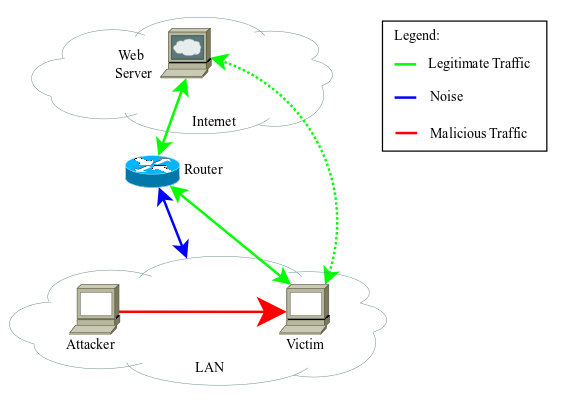
\includegraphics[width=9cm]{../figures/fig09.png}
	     \caption{Scenario to reproduce legitimate traffic, noise, flood and port scan.}
	     \label{fig:2_fig1}
	\end{figure}

\end{frame}
%-=-=-=-=-=-=-=-=-=-=-=-=-=-=-=-=-=-=-=-=-=-=-=-=
%	FRAME: Synthetic Dataset
%-=-=-=-=-=-=-=-=-=-=-=-=-=-=-=-=-=-=-=-=-=-=-=-=
\begin{frame}[c]{Synthetic Dataset}
	
	\begin{figure}[h!]
	     \centering 
	     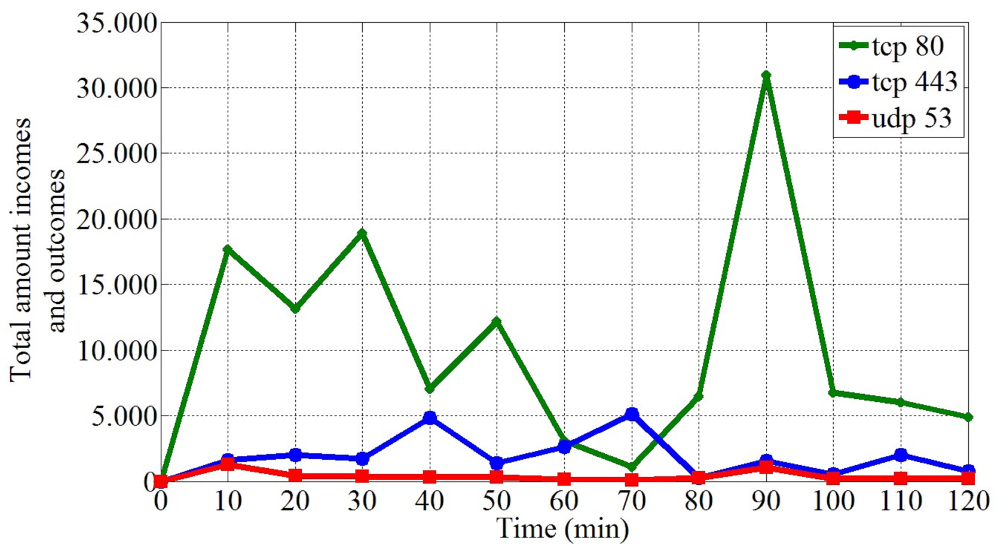
\includegraphics[width=9cm]{../figures/fig03.png}
	     \caption{Traffic from user's operations, that can be characterized by web access, traffic of well-known applications or network protocols.}
	     \label{fig:2_fig3}
	\end{figure}

\end{frame}
%-=-=-=-=-=-=-=-=-=-=-=-=-=-=-=-=-=-=-=-=-=-=-=-=
%	FRAME: Synthetic Dataset
%-=-=-=-=-=-=-=-=-=-=-=-=-=-=-=-=-=-=-=-=-=-=-=-=
% \begin{frame}[c]{Synthetic Dataset}
	
% 	\begin{figure}[h!]
% 	     \centering 
% 	     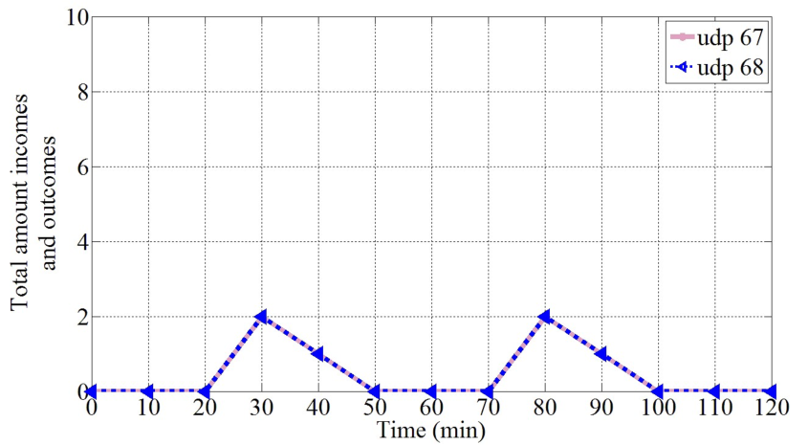
\includegraphics[width=9cm]{../figures/fig04.png}
% 	     \caption{Network traffic of user independent operations for network management.}
% 	     \label{fig:2_fig4}
% 	\end{figure}

% \end{frame}
%-=-=-=-=-=-=-=-=-=-=-=-=-=-=-=-=-=-=-=-=-=-=-=-=
%	FRAME: Synthetic Dataset
%-=-=-=-=-=-=-=-=-=-=-=-=-=-=-=-=-=-=-=-=-=-=-=-=
\begin{frame}[c]{Synthetic Dataset}
	
	\begin{figure}[h!]
	     \centering 
	     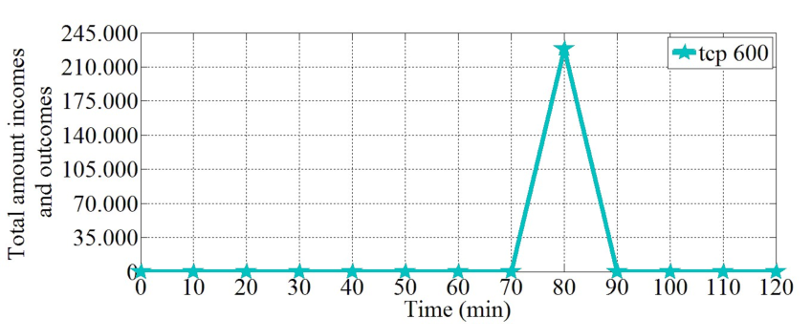
\includegraphics[width=9cm]{../figures/fig05.png}
	     \caption{A large quantity of SYN requests to a target, in order to cause a DoS.}
	     \label{fig:2_fig5}
	\end{figure}

\end{frame}
% %-=-=-=-=-=-=-=-=-=-=-=-=-=-=-=-=-=-=-=-=-=-=-=-=
% %	FRAME: Synthetic Dataset
% %-=-=-=-=-=-=-=-=-=-=-=-=-=-=-=-=-=-=-=-=-=-=-=-=
% \begin{frame}[c]{Synthetic Dataset}
	
% 	\begin{figure}[h!]
% 	     \centering 
% 	     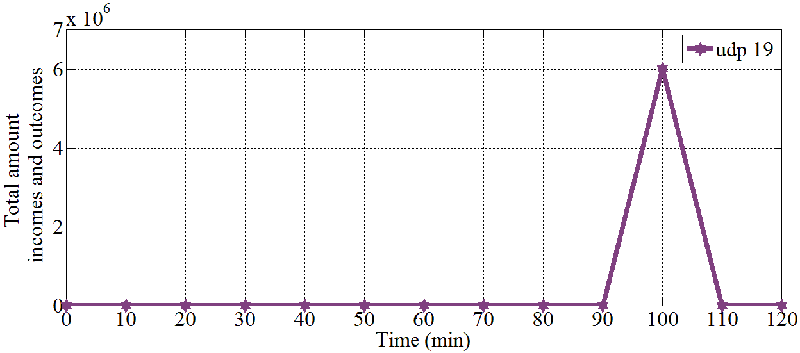
\includegraphics[width=9cm]{../figures/fig06.png}
% 	     \caption{Large amount of “UDP echo” requests and replies, causing packet flooding.}
% 	     \label{fig:2_fig6}
% 	\end{figure}

% \end{frame}
% %-=-=-=-=-=-=-=-=-=-=-=-=-=-=-=-=-=-=-=-=-=-=-=-=
% %	FRAME: Synthetic Dataset
% %-=-=-=-=-=-=-=-=-=-=-=-=-=-=-=-=-=-=-=-=-=-=-=-=
% \begin{frame}[c]{Synthetic Dataset}
	
% 	\begin{figure}[h!]
% 	     \centering 
% 	     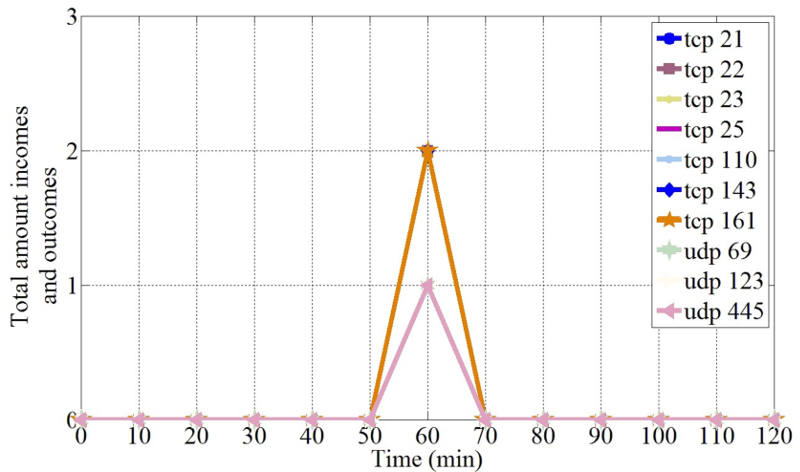
\includegraphics[width=9cm]{../figures/fig07.png}
% 	     \caption{Connection attempts in order to identify active ports.}
% 	     \label{fig:2_fig7}
% 	\end{figure}

% \end{frame}
%-=-=-=-=-=-=-=-=-=-=-=-=-=-=-=-=-=-=-=-=-=-=-=-=
%	FRAME: DARPA Dataset
%-=-=-=-=-=-=-=-=-=-=-=-=-=-=-=-=-=-=-=-=-=-=-=-=
\begin{frame}{DARPA Dataset}
	
	\begin{itemize}
		\item \textbf{7 weeks} of sniffed traffic saved into raw TCPDUMP packet data, from \textbf{inside and outside} origins, with \textbf{labeled} attacks;
		\item The most cases of \textbf{DoS focus on exploit} system vulnerabilities instead of on \textbf{flooding} attack;
		\item We select the cases that reproduce \textbf{probe and flooding} attacks.
	\end{itemize}

\end{frame}
%-=-=-=-=-=-=-=-=-=-=-=-=-=-=-=-=-=-=-=-=-=-=-=-=
%	FRAME: Proposed Framework
%-=-=-=-=-=-=-=-=-=-=-=-=-=-=-=-=-=-=-=-=-=-=-=-=
\begin{frame}{Proposed Framework}
	
	\begin{figure}[h!]
		\centering
	     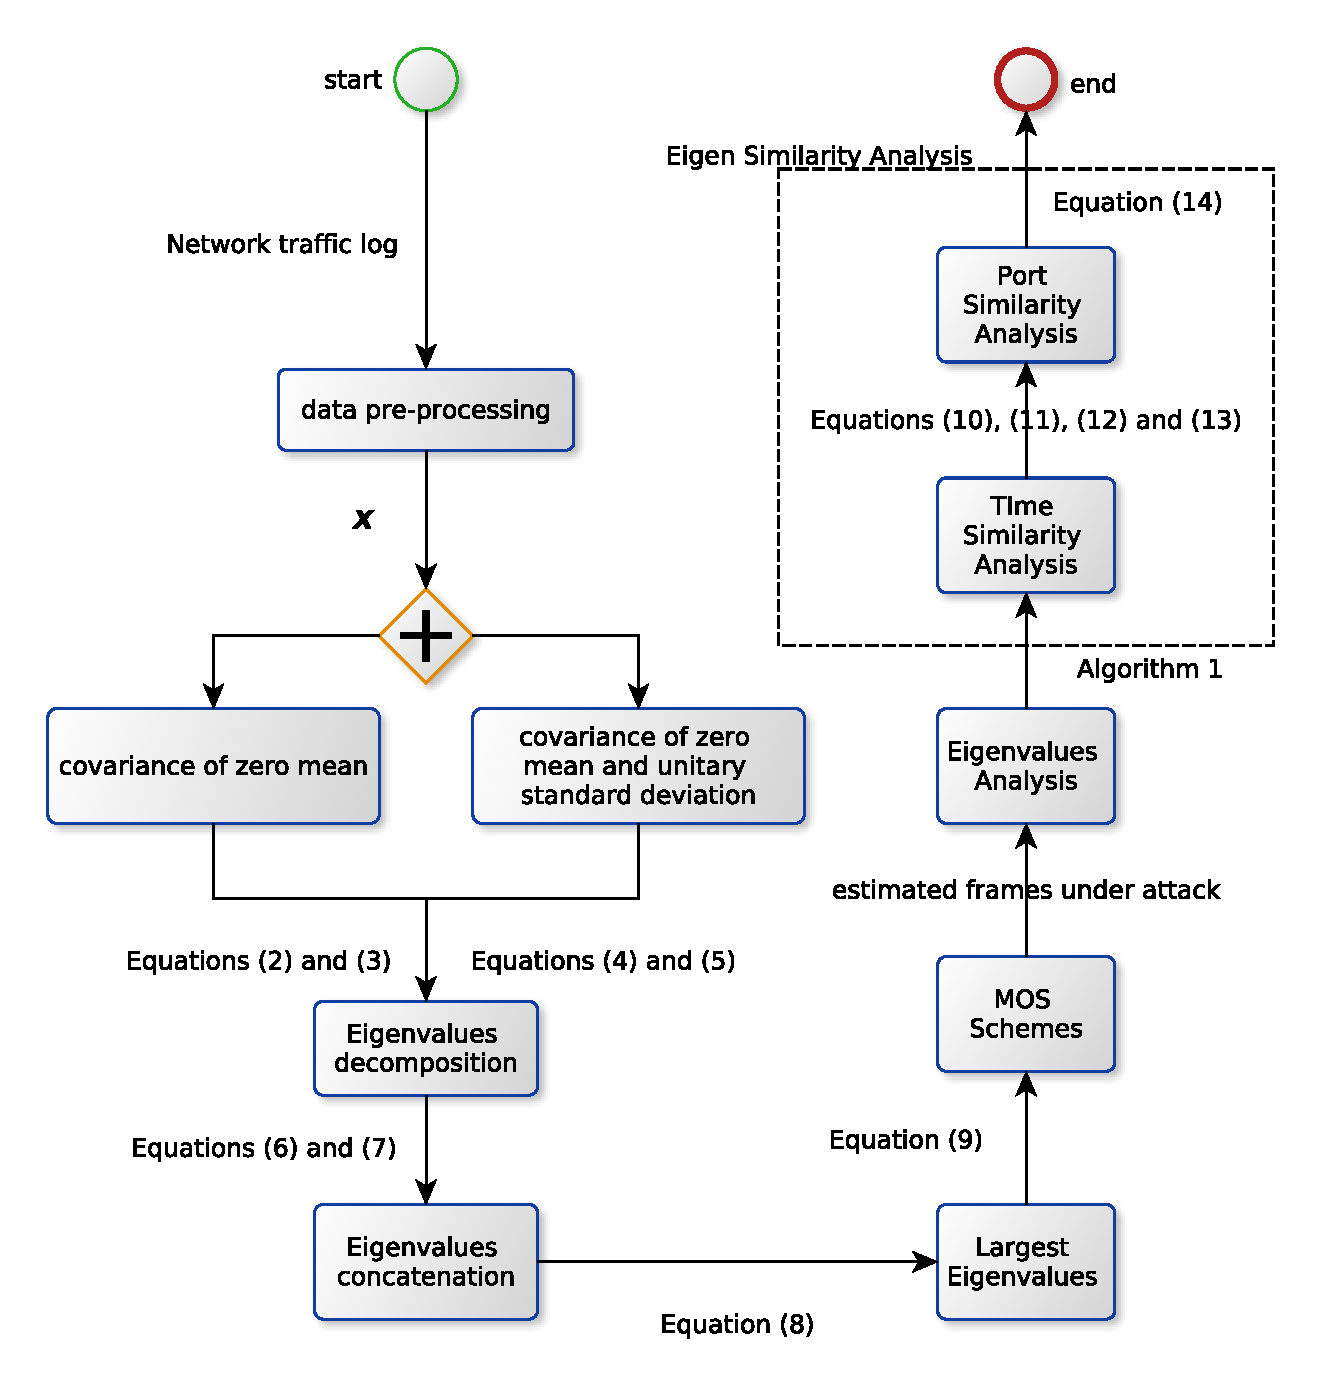
\includegraphics[width=7cm]{../figures/mos_eigen_similarity.eps}
	     \caption{Overview of The Framework for Detection and Identification of Network Attacks.}
	     \label{fig:2_fig80}
	\end{figure}

\end{frame}
% %-=-=-=-=-=-=-=-=-=-=-=-=-=-=-=-=-=-=-=-=-=-=-=-=
% %	FRAME: Proposed Framework
% %-=-=-=-=-=-=-=-=-=-=-=-=-=-=-=-=-=-=-=-=-=-=-=-=
% \begin{frame}{Proposed Framework}
	
% 	For \textbf{flooding} detection, calculate the \textbf{sample covariance matrix} $\boldsymbol{\hat{R}}_{yy}^{(q)}$ of the zero mean samples given by
% 	\begin{equation}\label{eq:eq02}
% 		\boldsymbol{y}_{m}^{(q)} = \boldsymbol{x}_{m}^{(q)} - \bar{\boldsymbol{x}}_{m}^{(q)}.
% 	\end{equation}

% 	the sample covariance matrix $\boldsymbol{\hat{R}}_{yy}^{(q)}$ can be calculated as follows
% 	\begin{equation}\label{eq:eq03}
% 		\boldsymbol{\hat{R}}_{yy}^{(q)} = \frac{1}{N}\boldsymbol{Y}^{(q)}\boldsymbol{Y}^{(q)^{\rm T}}.
% 	\end{equation}

% \end{frame}
% %-=-=-=-=-=-=-=-=-=-=-=-=-=-=-=-=-=-=-=-=-=-=-=-=
% %	FRAME: Proposed Framework
% %-=-=-=-=-=-=-=-=-=-=-=-=-=-=-=-=-=-=-=-=-=-=-=-=
% \begin{frame}{Proposed Framework}
	
% 	For \textbf{probing} detection, compute the \textbf{sample covariance} $\boldsymbol{\hat{R}}_{zz}^{(q)}$ whose variables have \textbf{zero mean and unitary standard deviation} as follows
% 	\begin{equation}\label{eq:eq04}
% 		\boldsymbol{z}_{m}^{(q)} = \frac{\boldsymbol{x}_{m}^{(q)} - \bar{\boldsymbol{x}}_{m}^{(q)}}{\boldsymbol{\sigma}_{m}^{(q)}}.
% 	\end{equation}

% 	The sample covariance matrix $\boldsymbol{\hat{R}}_{zz}^{(q)}$ can be calculated via 
% 	\begin{equation}\label{eq:eq05}
% 		\boldsymbol{\hat{R}}_{zz}^{(q)} = \frac{1}{N}\boldsymbol{Z}^{(q)}\boldsymbol{Z}^{(q)^{\rm T}}.
% 	\end{equation}

% \end{frame}
% %-=-=-=-=-=-=-=-=-=-=-=-=-=-=-=-=-=-=-=-=-=-=-=-=
% %	FRAME: Proposed Framework
% %-=-=-=-=-=-=-=-=-=-=-=-=-=-=-=-=-=-=-=-=-=-=-=-=
% \begin{frame}{Proposed Framework}
	
% 	we refer to $\boldsymbol{\hat{R}}_{yy}$ and $\boldsymbol{\hat{R}}_{zz}$ as a matrix $\boldsymbol{C}$

% 	Compute eigenvalue decomposition (EVD) to obtain the vector of eigenvalues $\boldsymbol{e}^{(q)}$ associated with each matrix (time frame $q$), according to (\ref{eq:eq060}).
% 	\begin{equation}\label{eq:eq06}
% 	\boldsymbol{C}^{(q)} = \boldsymbol{V}^{(q)}\boldsymbol{\Lambda}^{(q)}\boldsymbol{V}^{(q)^{\rm T}},
% 	\end{equation}
% 	\begin{equation}\label{eq:eq060}
% 	\boldsymbol{e}^{(q)} = \rm diag(\boldsymbol{\Lambda}^{(q)}),
% 	\end{equation}

% 	The eigenvalues should be sorted in descending order, i.e., $\lambda_{1}^{(q)} > \lambda_{2}^{(q)} > \lambda_{3}^{(q)} > ... > \lambda_{m}^{(q)}$.

% \end{frame}
% %-=-=-=-=-=-=-=-=-=-=-=-=-=-=-=-=-=-=-=-=-=-=-=-=
% %	FRAME: Proposed Framework
% %-=-=-=-=-=-=-=-=-=-=-=-=-=-=-=-=-=-=-=-=-=-=-=-=
% \begin{frame}{Proposed Framework}
	
% 	\begin{equation}\label{eq:eq07}
% 		\boldsymbol{E} =
% 		\begin{bmatrix}
% 			\color{red}\lambda_1^{(1)} & \color{red}\lambda_1^{(2)} & \color{red}\lambda_1^{(3)} & \cdots & \color{red}\lambda_1^{(Q)} \\
% 			\lambda_2^{(1)} & \lambda_2^{(2)} & \lambda_2^{(3)} & \cdots & \lambda_2^{(Q)} \\
% 			\lambda_3^{(1)} & \lambda_3^{(2)} & \lambda_3^{(3)} & \cdots & \lambda_3^{(Q)} \\
% 			\vdots & \vdots & \ddots & \vdots  \\
% 			\lambda_m^{(1)} & \lambda_m^{(2)} & \lambda_m^{(3)} & \cdots & \lambda_m^{(Q)} \\
% 		\end{bmatrix}.
% 	\end{equation}

% 	\begin{equation}\label{eq:eq08}
% 		\boldsymbol{e}_{\rm max} = \boldsymbol{E}\{:,1\} = [ \lambda_1^{(1)}, \lambda_1^{(2)} ... \lambda_1^{(Q)}]
% 	\end{equation}

% \end{frame}
% %-=-=-=-=-=-=-=-=-=-=-=-=-=-=-=-=-=-=-=-=-=-=-=-=
% %	FRAME: MOS Scheme
% %-=-=-=-=-=-=-=-=-=-=-=-=-=-=-=-=-=-=-=-=-=-=-=-=
% \begin{frame}{MOS Scheme}

% 	\begin{itemize}
% 		\item Traditionally the MOS schemes are applied for the eigenvalues of the vector $\boldsymbol{e}^{(q)}$;
% 		\item $\boldsymbol{e}_{\rm max}$ is sorted in descending order, producing $\sim\boldsymbol{e}_{\rm max}$, that is used as input parameter for MOS schemes, according to $\hat{d} = \rm{MOS}(\sim\boldsymbol{e}_{\rm max})$.
% 		\item $\hat{d}$ is the estimated number of time frames under attack.
% 	\end{itemize}
	
% \end{frame}
%-=-=-=-=-=-=-=-=-=-=-=-=-=-=-=-=-=-=-=-=-=-=-=-=
%	FRAME: Eigenvalue Analysis
%-=-=-=-=-=-=-=-=-=-=-=-=-=-=-=-=-=-=-=-=-=-=-=-=
\begin{frame}{Eigenvalue Analysis}
	
	\textbf{MOS} reveal the \textbf{number of attacks} and through \textbf{eigenvalue analysis} we identify the \textbf{time frames} $q$ under attack

	\begin{figure}[h!]
	     \centering 
	     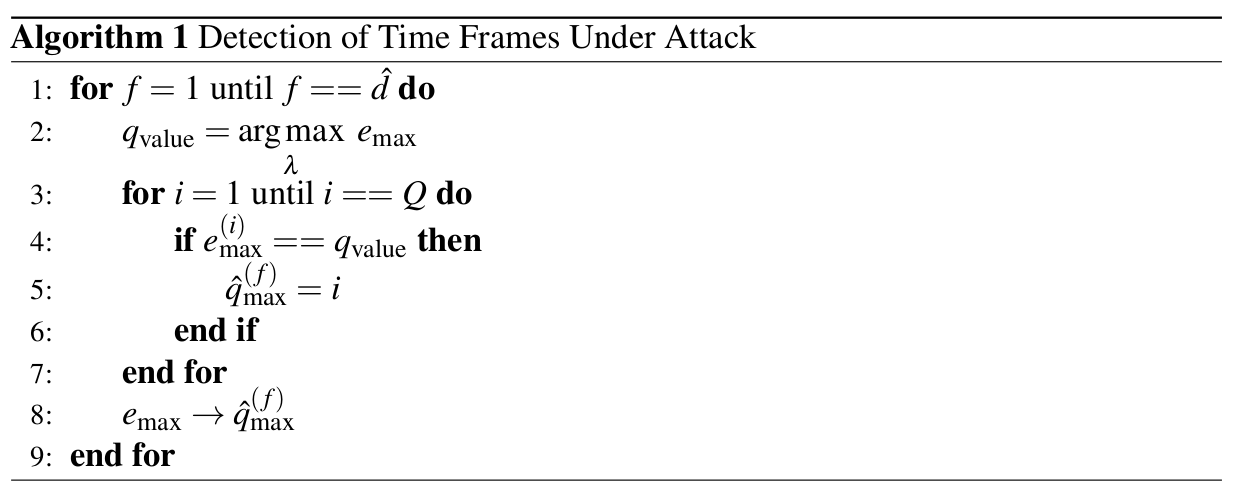
\includegraphics[width=11cm]{alg.png}
	     \label{fig:2_fig91}
	\end{figure}

\end{frame}
%-=-=-=-=-=-=-=-=-=-=-=-=-=-=-=-=-=-=-=-=-=-=-=-=
%	FRAME: Eigenvalue Analysis
%-=-=-=-=-=-=-=-=-=-=-=-=-=-=-=-=-=-=-=-=-=-=-=-=
\begin{frame}{Eigen Similarity Analysis}
	
	\textbf{Eigen Similarity} Analysis attempts to identify \textbf{time and ports}.

	The \textbf{reference eigenvectors} $\boldsymbol{v}^{(q)}$ is calculated from the \textbf{traffic without attack}.

	Each $\boldsymbol{x}^{(\hat{q})}_{(n)}$ vector of each $n$-th minutes of the estimated $\rm{\boldsymbol{\hat{q}}}_{\rm max}$ time frames shall be individually appended into $\boldsymbol{X}^{(q)}$
	\begin{equation}\label{eq:eq12}
		\boldsymbol{X}_{n} = \{\boldsymbol{X}^{(q)} | \boldsymbol{x}^{(\hat{q})}_{(n)}\}.
	\end{equation}

	The resultant $\boldsymbol{X}_{(n)}$ is necessary to obtain $\boldsymbol{v}_{(n)}$

\end{frame}
%-=-=-=-=-=-=-=-=-=-=-=-=-=-=-=-=-=-=-=-=-=-=-=-=
%	FRAME: Eigenvalue Analysis
%-=-=-=-=-=-=-=-=-=-=-=-=-=-=-=-=-=-=-=-=-=-=-=-=
\begin{frame}{Eigen Similarity Analysis}
	
	$s_n$ denotes the absolute similarity degree of the $n$-th minute
	
	$\boldsymbol{v}^{(q)}$ is the most significant eigenvectors

	$\boldsymbol{v}_{(n)}$ is the most significant eigenvectors obtained after append the target $n$-th minute of one network traffic

	we evaluate the cosine similarity to identify legitimate and malicious traffic,
	\begin{equation}
		\label{eq:eq11}
		s_n = \frac{\abs{\boldsymbol{v}^{(q)} \cdot \boldsymbol{v}_{(n)}}}{\norm{\boldsymbol{v}^{(q)}}\norm{\boldsymbol{v}_{(n)}}},
	\end{equation}

\end{frame}
%-=-=-=-=-=-=-=-=-=-=-=-=-=-=-=-=-=-=-=-=-=-=-=-=
%	FRAME: Eigenvalue Analysis
%-=-=-=-=-=-=-=-=-=-=-=-=-=-=-=-=-=-=-=-=-=-=-=-=
\begin{frame}{Eigen Similarity Analysis}
	
	We propose and evaluate \textbf{three approaches} for eigen similarity analysis: 
	\begin{itemize}
		\item \textbf{incremental:} concatenates eigenvectors incrementally;
		\item \textbf{individual:} concatenates each eigenvector individually and discards;
		\item \textbf{incremental individualized:} incremental until detect attach and individual after.
	\end{itemize}

\end{frame}
%-=-=-=-=-=-=-=-=-=-=-=-=-=-=-=-=-=-=-=-=-=-=-=-=
%	FRAME: Eigenvalue Analysis
%-=-=-=-=-=-=-=-=-=-=-=-=-=-=-=-=-=-=-=-=-=-=-=-=
\begin{frame}{Eigen Similarity Analysis}
	
	\begin{figure}[h!]
		\centering
	    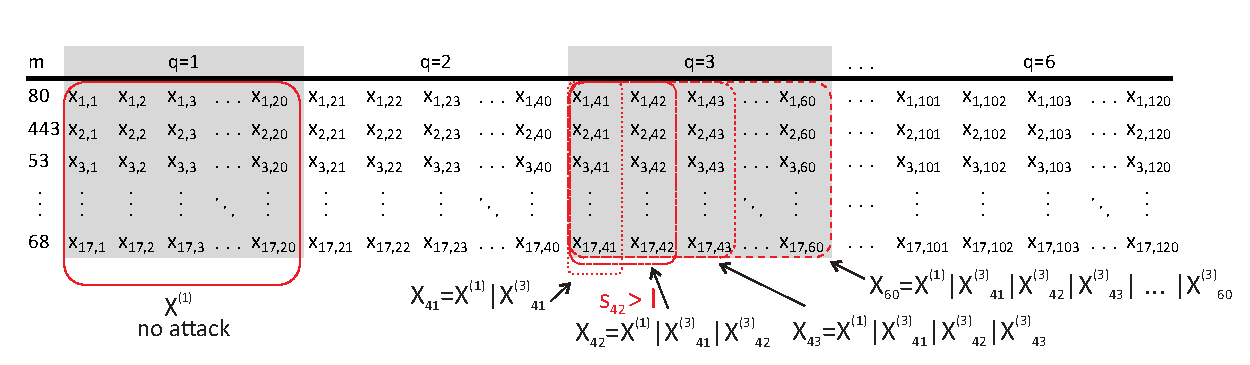
\includegraphics[width=11.5cm]{../figures/incremental.eps}
	    \caption{Traffic selection for incremental approach.}
	    \label{fig:2_fig8}
	\end{figure}

\end{frame}
%-=-=-=-=-=-=-=-=-=-=-=-=-=-=-=-=-=-=-=-=-=-=-=-=
%	FRAME: Eigenvalue Analysis
%-=-=-=-=-=-=-=-=-=-=-=-=-=-=-=-=-=-=-=-=-=-=-=-=
\begin{frame}{Eigen Similarity Analysis}
	
	\begin{figure}[h!]
	     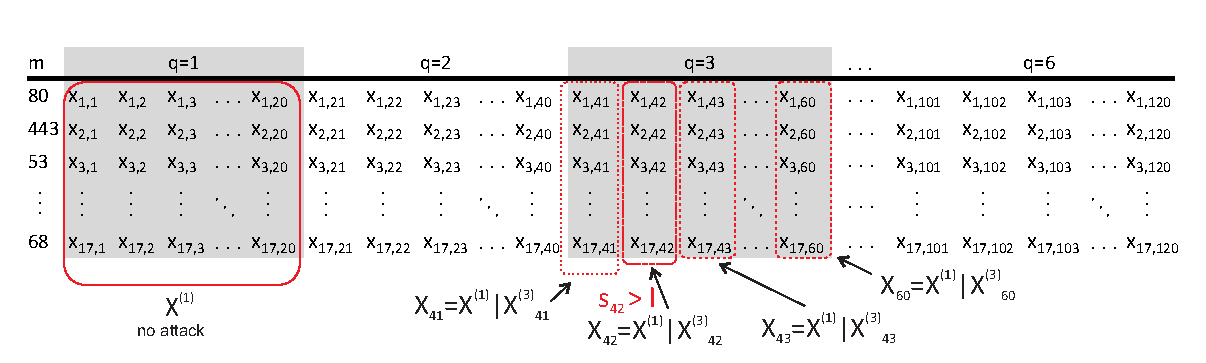
\includegraphics[width=11.5cm]{../figures/individualized.eps}
	     \caption{Traffic selection for individual approach.}
	     \label{fig:2_fig9}
	\end{figure}
\end{frame}
%-=-=-=-=-=-=-=-=-=-=-=-=-=-=-=-=-=-=-=-=-=-=-=-=
%	FRAME: Eigenvalue Analysis
%-=-=-=-=-=-=-=-=-=-=-=-=-=-=-=-=-=-=-=-=-=-=-=-=
\begin{frame}{Eigen Similarity Analysis}
	
	\begin{figure}[h!]
	     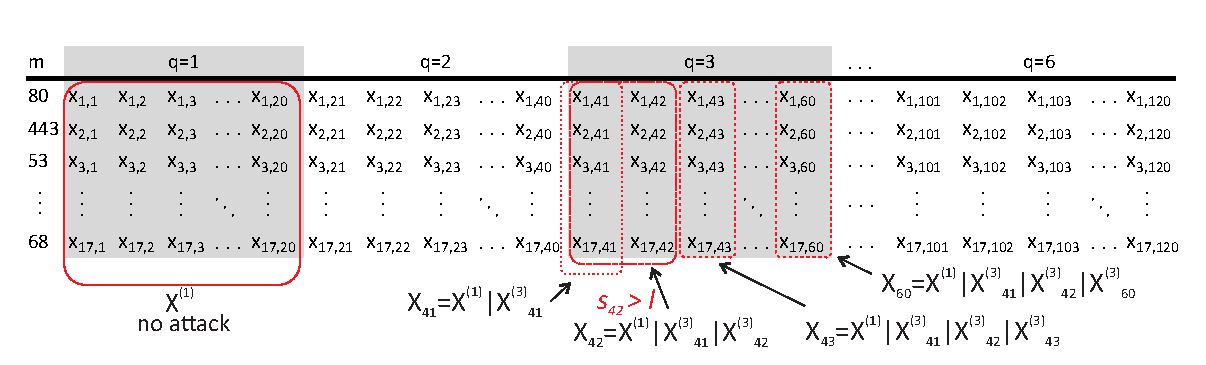
\includegraphics[width=11.5cm]{../figures/incremental_individualized.eps}
	     \caption{Traffic selection for incremental individualized approach.}
	     \label{fig:2_fig2}
	\end{figure}

\end{frame}
%-=-=-=-=-=-=-=-=-=-=-=-=-=-=-=-=-=-=-=-=-=-=-=-=
%	FRAME: Eigenvalue Analysis
%-=-=-=-=-=-=-=-=-=-=-=-=-=-=-=-=-=-=-=-=-=-=-=-=
\begin{frame}{Eigen Similarity Analysis}
	
	\textbf{For detection of ports under attack}, the $\boldsymbol{v}^{(q)}$ last most significant eigenvectors without attack is compared against the $\boldsymbol{v}_{(n)}$ identified as under attack, 

	Evaluate the cosine similarity of each $m$-th port of all $\boldsymbol{\hat{n}}$ minutes.

	\begin{equation}\label{eq:eq15}
		\left\{
		\begin{array}{@{}ll@{}}
			x_{(m,n)} = x^{(\hat{q})}_{(m,\hat{n})} \\
			\\
			s_{m,\hat{n}} = \frac{\abs{\boldsymbol{v}^{(q)} \cdot \boldsymbol{v}_{(m,\hat{n})}}}{\norm{\boldsymbol{v}^{(q)}}\norm{\boldsymbol{v}_{(m,\hat{n})}}},
		\end{array}\right.
	\end{equation}

\end{frame}
% %-=-=-=-=-=-=-=-=-=-=-=-=-=-=-=-=-=-=-=-=-=-=-=-=
% %	FRAME: Results
% %-=-=-=-=-=-=-=-=-=-=-=-=-=-=-=-=-=-=-=-=-=-=-=-=
% \begin{frame}{Results}
	
% 	\begin{table}[h!]
% 	  \centering
% 	  \scriptsize
% 	  \caption{Largest Eigenvalue related to attacks detection}
% 	  \label{tab:tab3}
% 	  \begin{tabular}{ c c c c c }
% 		\toprule
% 		\multirow{3}{*}{\textbf{Time Frame} $q$} &\multicolumn{4}{c }{\textbf{Vectors GETV}}\\ 
% 				\hhline{~----}
% 			&\textbf{Detection of}	 &\textbf{Detection of}	 &\textbf{Detection of}	 &\textbf{Detection of}\\
% 			&\textbf{\emph{synflood/fraggle}}	 &\textbf{\emph{synflood}}	 &\textbf{\emph{fraggle}}	 &\textbf{\emph{port scan}}\\
% 		\midrule
% 		1 &1887545 &1887545 &1887545 &2,0734 \\
% 		2 &2341327 &2341327 &2341327 &2,1451 \\
% 		3 &3213867 &3213867 &3213867 &\color{red}10,0718 \\
% 		4 &\color{red}133238294 &\color{red}133238294 &731229 &2,1620 \\
% 		5 &\color{red}92384021611 &6367983 &\color{red}92384021611 &2,4253 \\
% 		6 &708335 &708335 &708335 &1,7948 \\
% 	    \bottomrule
% 	  \end{tabular}
% 	\end{table}

% \end{frame}
% %-=-=-=-=-=-=-=-=-=-=-=-=-=-=-=-=-=-=-=-=-=-=-=-=
% %	FRAME: Results
% %-=-=-=-=-=-=-=-=-=-=-=-=-=-=-=-=-=-=-=-=-=-=-=-=
% \begin{frame}{Results}
	
% 	\begin{table}[h!]
% 	  \centering
% 	  \tiny
% 	  \caption{MOS schemes applied to port scan and flood detection}
% 	  \label{tab:tab4}
% 	  \begin{tabular}{ c c c c c c c c }
% 		\toprule
% 		\multirow{2}{*}{\textbf{Type of analysis} $q$} &\multicolumn{6}{c}{\textbf{MOS schemes (estimated model order $\hat{d}$)}} &{\textbf{(d)}}\\ 
% 				\hhline{~------~}
% 			&\textbf{AIC} &\textbf{MDL} &\textbf{EDC} &\textbf{RADOI} &\textbf{EFT} &\textbf{SURE}\\
% 		\midrule
% 		Detection of synflood \\(presence of attack) &2 &1 &\textbf{\color{red}1} &5 &\textbf{\color{red}1} &4 &\textbf{\color{red}1} \\
% 		Detection of synflood \\(absence of attack) &1 &1 &\textbf{\color{red}0} &1 &\textbf{\color{red}0} &3 &\textbf{\color{red}0} \\
% 		\midrule
% 		Detection of fraggle \\(presence of attack) &1 &1 &\textbf{\color{red}1} &5 &\textbf{\color{red}1} &4 &\textbf{\color{red}1} \\
% 		Detection of fraggle \\(absence of attack) &1 &1 &\textbf{\color{red}0} &1 &\textbf{\color{red}0} &3 &\textbf{\color{red}0} \\
% 		\midrule
% 		Detection of port scan \\(presence of attack) &1 &1 &\textbf{\color{red}1} &1 &\textbf{\color{red}1} &9 &\textbf{\color{red}1} \\
% 		Detection of port scan \\(absence of attack) &0 &0 &\textbf{\color{red}0} &1 &\textbf{\color{red}0} &1 &\textbf{\color{red}0} \\
% 		\midrule
% 		Detection of synflood/fraggle \\(presence of attack) &2 &2 &\textbf{\color{red}2} &5 &\textbf{\color{red}2} &5 &\textbf{\color{red}2} \\
% 		Detection of synflood/fraggle \\(absence of attack) &1 &1 &\textbf{\color{red}0} &1 &\textbf{\color{red}0} &3 &\textbf{\color{red}0} \\
% 	    \bottomrule
% 	  \end{tabular}
% 	\end{table}

% \end{frame}
% %-=-=-=-=-=-=-=-=-=-=-=-=-=-=-=-=-=-=-=-=-=-=-=-=
% %	FRAME: Results
% %-=-=-=-=-=-=-=-=-=-=-=-=-=-=-=-=-=-=-=-=-=-=-=-=
% \begin{frame}{Results}
	
% 	MOS schemes for probing and flooding attack detection:
% 	\begin{itemize}
% 		\item The \textbf{largest eigenvalues visually} indicate the time frame under probing and flooding attack detection;
% 		\item MOS schemes can estimate it mathematically;
% 		\begin{itemize}
% 			\item \textbf{EDC and EFT} estimate \textbf{correctly} the number of attacks $d$;
% 		\end{itemize}
% 	\end{itemize}

% 	It is still necessary \textbf{to identify} the \textbf{times and ports} under attack.

% \end{frame}
%-=-=-=-=-=-=-=-=-=-=-=-=-=-=-=-=-=-=-=-=-=-=-=-=
%	FRAME: Results
%-=-=-=-=-=-=-=-=-=-=-=-=-=-=-=-=-=-=-=-=-=-=-=-=
\begin{frame}{Results}
	
	\begin{table}[h!]
	  \centering
	  \tiny
	  \caption{Eigen Similarity Analysis for Port Scan Detection}
	  \label{tab:tab5}
	  \begin{tabular}{ c c c c c c }
		\toprule
		\multirow{2}{*}{\textbf{Time Frame} $q$} &\multirow{2}{*}{\textbf{Time} $n$}   &\multicolumn{3}{c}{\textbf{Similarity Analysis}} &\multirow{2}{*}{\textbf{Attack?}}\\ 
				\hhline{~~---~}
				& &\textbf{Incremental Individualized} &\textbf{Incremental} &\textbf{Individual}\\
		\midrule
		3 &1 &0.9946 &0.9946 &0.9946 &no \\
		3 &2 &0.9934 &0.9934 &0.9999 &no \\
		3 &3 &0.9912 &0.9912 &0.9999 &no \\
		3 &4 &0.9888 &0.9888 &0.9999 &no \\
		3 &5 &0.9856 &0.9856 &0.9998 &no \\
		3 &6 &0.9840 &0.9840 &0.9999 &no \\
		3 &7 &0.9824 &0.9824 &1.0000 &no \\
		3 &8 &0.9794 &0.9794 &0.9999 &no \\
		3 &9 &0.9673 &0.9673 &0.9926 &no \\
		3 &10 &0.9674 &0.9674 &0.9997 &no \\
		3 &11 &0.9733 &0.9733 &0.9993 &no \\
		3 &12 &0.9702 &0.9702 &0.9993 &no \\
		3 &13 &0.9677 &0.9677 &0.9999 &no \\
		3 &14 &0.9646 &0.9646 &0.9998 &no \\
		3 &15 &\color{red}0.0216 &\color{red}0.0216 &\color{red}0.0276 &\color{red}yes \\
		3 &16 &0.9621 &\color{red}0.0209 &1.0000 &no \\
		3 &17 &0.9611 &\color{red}0.0199 &0.9998 &no \\
		3 &18 &0.9612 &\color{red}0.0191 &0.9999 &no \\
		3 &19 &0.9613 &\color{red}0.0186 &0.9998 &no \\
		3 &20 &0.9638 &\color{red}0.0190 &1.0000 &no \\
	    \bottomrule
	  \end{tabular}
	\end{table}	
	
\end{frame}
%-=-=-=-=-=-=-=-=-=-=-=-=-=-=-=-=-=-=-=-=-=-=-=-=
%	FRAME: Results
%-=-=-=-=-=-=-=-=-=-=-=-=-=-=-=-=-=-=-=-=-=-=-=-=
\begin{frame}{Results}
	
	\begin{table}[h!]
	  \centering
	  \tiny
	  \caption{Eigen Similarity Analysis for Synflood Detection}
	  \label{tab:tab6}
	  \begin{tabular}{ c c c c c c }
		\toprule
		\multirow{2}{*}{\textbf{Time Frame} $q$} &\multirow{2}{*}{\textbf{Time} $n$}   &\multicolumn{3}{c}{\textbf{Similarity Analysis}} &\multirow{2}{*}{\textbf{Attack?}}\\ 
				\hhline{~~---~}
				& &\textbf{Incremental Individualized} &\textbf{Incremental} &\textbf{Individual}\\
		\midrule
		4 &1 &1.0000 &1.0000 &1.0000 &no \\
		4 &2 &0.9999 &0.9999 &1.0000 &no \\
		4 &3 &0.9997 &0.9997 &0.9999 &no \\
		4 &4 &0.9998 &0.9998 &1.0000 &no \\
		4 &5 &0.9965 &0.9965 &0.9908 &no \\
		4 &6 &0.9975 &0.9975 &1.0000 &no \\
		4 &7 &0.9977 &0.9977 &1.0000 &no \\
		4 &8 &0.9980 &0.9980 &1.0000 &no \\
		4 &9 &0.9987 &0.9987 &0.9999 &no \\
		4 &10 &0.9991 &0.9991 &1.0000 &no \\
		4 &11 &\color{red}0.0085 &\color{red}0.0085 &\color{red}0.0284 &\color{red}yes \\
		4 &12 &\color{red}0.0162 &\color{red}0.0120 &\color{red}0.0343 &\color{red}yes \\
		4 &13 &\color{red}0.0248 &\color{red}0.0158 &\color{red}0.0427 &\color{red}yes \\
		4 &14 &\color{red}0.1243 &\color{red}0.0185 &\color{red}0.1041 &\color{red}yes \\
		4 &15 &\color{red}0.0082 &\color{red}0.0162 &\color{red}0.0103 &\color{red}yes \\
		4 &16 &\color{red}0.0404 &\color{red}0.0070 &\color{red}0.0580 &\color{red}yes \\
		4 &17 &\color{red}0.0397 &\color{red}0.0007 &\color{red}0.0573 &\color{red}yes \\
		4 &18 &\color{red}0.0408 &\color{red}0.0042 &\color{red}0.0584 &\color{red}yes \\
		4 &19 &\color{red}0.0408 &\color{red}0.0079 &\color{red}0.0584 &\color{red}yes \\
		4 &20 &\color{red}0.0477 &\color{red}0.0092 &\color{red}0.0757 &\color{red}yes \\
	    \bottomrule
	  \end{tabular}
	\end{table}	
	
\end{frame}
%-=-=-=-=-=-=-=-=-=-=-=-=-=-=-=-=-=-=-=-=-=-=-=-=
%	FRAME: Results
%-=-=-=-=-=-=-=-=-=-=-=-=-=-=-=-=-=-=-=-=-=-=-=-=
\begin{frame}{Results}
	
	\begin{table}[h!]
	  \centering
	  \tiny
	  \caption{Eigen Similarity Analysis for Fraggle Detection}
	  \label{tab:tab7}
	  \begin{tabular}{ c c c c c c }
		\toprule
		\multirow{2}{*}{\textbf{Time Frame} $q$} &\multirow{2}{*}{\textbf{Time} $n$}   &\multicolumn{3}{c}{\textbf{Similarity Analysis}} &\multirow{2}{*}{\textbf{Attack?}}\\ 
				\hhline{~~---~}
				& &\textbf{Incremental Individualized} &\textbf{Incremental} &\textbf{Individual}\\
		\midrule
		5 &1 &1.0000 &1.0000 &1.0000 &no \\
		5 &2 &0.9999 &0.9999 &1.0000 &no \\
		5 &3 &1.0000 &1.0000 &1.0000 &no \\
		5 &4 &0.9999 &0.9999 &1.0000 &no \\
		5 &5 &0.9993 &0.9993 &0.9997 &no \\
		5 &6 &0.9993 &0.9993 &0.9997 &no \\
		5 &7 &0.9994 &0.9994 &1.0000 &no \\
		5 &8 &0.9995 &0.9995 &1.0000 &no \\
		5 &9 &0.9995 &0.9995 &1.0000 &no \\
		5 &10 &0.9995 &0.9995 &1.0000 &no \\
		5 &11 &\color{red}0.0031 &\color{red}0.0031 &\color{red}0.0021 &\color{red}yes \\
		5 &12 &\color{red}0.0019 &\color{red}0.0025 &\color{red}0.0009 &\color{red}yes \\
		5 &13 &\color{red}0.0030 &\color{red}0.0026 &\color{red}0.0020 &\color{red}yes \\
		5 &14 &\color{red}0.0030 &\color{red}0.0027 &\color{red}0.0020 &\color{red}yes \\
		5 &15 &\color{red}0.0030 &\color{red}0.0028 &\color{red}0.0020 &\color{red}yes \\
		5 &16 &\color{red}0.0012 &\color{red}0.0025 &\color{red}0.0002 &\color{red}yes \\
		5 &17 &\color{red}0.0030 &\color{red}0.0026 &\color{red}0.0020 &\color{red}yes \\
		5 &18 &\color{red}0.0030 &\color{red}0.0026 &\color{red}0.0020 &\color{red}yes \\
		5 &19 &\color{red}0.0030 &\color{red}0.0027 &\color{red}0.0020 &\color{red}yes \\
		5 &20 &\color{red}0.0069 &\color{red}0.0023 &\color{red}0.0083 &\color{red}yes \\
	    \bottomrule
	  \end{tabular}
	\end{table}
	
\end{frame}
%-=-=-=-=-=-=-=-=-=-=-=-=-=-=-=-=-=-=-=-=-=-=-=-=
%	FRAME: Results
%-=-=-=-=-=-=-=-=-=-=-=-=-=-=-=-=-=-=-=-=-=-=-=-=
\begin{frame}{Results}
	
	\begin{table}[h!]
	  \centering
	  \tiny
	  \caption{Eigen Similarity Analysis for Detection of Ports Under Port Scan Attack (q=3 and n=15)}
	  \label{tab:tab8}
	  \begin{tabular}{ c c c c }
		\toprule
		\multirow{2}{*}{\textbf{Port} $p$}   &\multicolumn{2}{c}{\textbf{Approaches}} &\multirow{2}{*}{\textbf{Attack?}}\\ 
				\hhline{~--~}
				&\textbf{Incremental Individualized} &\textbf{Individual}\\
		\midrule
		80 &0.9999 &0.9999 &no \\
		443 &0.9999 &0.9999 &no \\
		53 &0.9999 &0.9999 &no \\
		21 &0.9999 &0.9997 &\color{red}yes \\
		22 &\color{red}0.0298 &0.9997 &\color{red}yes \\
		23 &\color{red}0.0298 &0.9997 &\color{red}yes \\
		25 &\color{red}0.0298 &0.9997 &\color{red}yes \\
		110 &\color{red}0.0298 &0.9997 &\color{red}yes \\
		143 &\color{red}0.0298 &0.9997 &\color{red}yes \\
		161 &\color{red}0.0298 &0.9997 &\color{red}yes \\
		69 &\color{red}0.0298 &0.9997 &\color{red}yes \\
		123 &\color{red}0.0298 &0.9997 &\color{red}yes \\
		445 &\color{red}0.0298 &0.9997 &\color{red}yes \\
		600 &0.9999 &0.9999 &no \\
		19 &0.9999 &0.9999 &no \\
		67 &0.9999 &0.9999 &no \\
		68 &0.9999 &0.9999 &no \\
	    \bottomrule
	  \end{tabular}
	\end{table}
	
\end{frame}
%-=-=-=-=-=-=-=-=-=-=-=-=-=-=-=-=-=-=-=-=-=-=-=-=
%	FRAME: Results
%-=-=-=-=-=-=-=-=-=-=-=-=-=-=-=-=-=-=-=-=-=-=-=-=
\begin{frame}{Results}
	
	\begin{table}[h!]
	  \centering
	  \tiny
	  \caption{Eigen Similarity Analysis for Detection of Ports Under Synflood Attack (q=4 and n=11)}
	  \label{tab:tab9}
	  \begin{tabular}{ c c c c }
		\toprule
		\multirow{2}{*}{\textbf{Port} $p$}   &\multicolumn{2}{c}{\textbf{Approaches}} &\multirow{2}{*}{\textbf{Attack?}}\\ 
				\hhline{~--~}
				&\textbf{Incremental Individualized} &\textbf{Individual}\\
		\midrule
		80 &1.0000 &1.0000 &no \\
		443 &1.0000 &1.0000 &no \\
		53 &1.0000 &1.0000 &no \\
		21 &1.0000 &1.0000 &nos \\
		22 &1.0000 &1.0000 &no \\
		23 &1.0000 &1.0000 &no \\
		25 &1.0000 &1.0000 &no \\
		110 &1.0000 &1.0000 &no \\
		143 &1.0000 &1.0000 &no \\
		161 &1.0000 &1.0000 &no \\
		69 &1.0000 &1.0000 &no \\
		123 &1.0000 &1.0000 &no \\
		445 &1.0000 &1.0000 &no \\
		600 &\color{red}0.0077 &\color{red}0.0427 &\color{red}yes \\
		19 &1.0000 &1.0000 &no \\
		67 &1.0000 &1.0000 &no \\
		68 &1.0000 &1.0000 &no \\
	    \bottomrule
	  \end{tabular}
	\end{table}
	
\end{frame}
%-=-=-=-=-=-=-=-=-=-=-=-=-=-=-=-=-=-=-=-=-=-=-=-=
%	FRAME: Results
%-=-=-=-=-=-=-=-=-=-=-=-=-=-=-=-=-=-=-=-=-=-=-=-=
\begin{frame}{Results}
	
	\begin{table}[h!]
	  \centering
	  \tiny
	  \caption{Eigen Similarity Analysis for Detection of Ports Under Fraggle Attack (q=5 and t=11)}
	  \label{tab:tab10}
	  \begin{tabular}{ c c c c }
		\toprule
		\multirow{2}{*}{\textbf{Port} $p$}   &\multicolumn{2}{c}{\textbf{Approaches}} &\multirow{2}{*}{\textbf{Attack?}}\\ 
				\hhline{~--~}
				&\textbf{Incremental Individualized} &\textbf{Individual}\\
		\midrule
		80 &1.0000 &1.0000 &no \\
		443 &1.0000 &1.0000 &no \\
		53 &1.0000 &1.0000 &no \\
		21 &1.0000 &1.0000 &no \\
		22 &1.0000 &1.0000 &no \\
		23 &1.0000 &1.0000 &no \\
		25 &1.0000 &1.0000 &no \\
		110 &1.0000 &1.0000 &no \\
		143 &1.0000 &1.0000 &no \\
		161 &1.0000 &1.0000 &no \\
		69 &1.0000 &1.0000 &no \\
		123 &1.0000 &1.0000 &no \\
		445 &1.0000 &1.0000 &no \\
		600 &1.0000 &1.0000 &no \\
		19 &\color{red}0.0031 &\color{red}0.0004 &\color{red}yes \\
		67 &1.0000 &1.0000 &no \\
		68 &1.0000 &1.0000 &no \\
	    \bottomrule
	  \end{tabular}
	\end{table}
	
\end{frame}
%-=-=-=-=-=-=-=-=-=-=-=-=-=-=-=-=-=-=-=-=-=-=-=-=
%	FRAME: Results
%-=-=-=-=-=-=-=-=-=-=-=-=-=-=-=-=-=-=-=-=-=-=-=-=
\begin{frame}{Results}
	
	For \textbf{time} attack detection:
	\begin{itemize}
		\item \textbf{High similarity} between network traffic \textbf{without attack} (0.9610) and \textbf{low similarity} with \textbf{attack} (0.0276);
		\item The \textbf{incremental} approach produces \textbf{false positive} results;
		\item Capability of \textbf{change detection} based on similarity between legitimate and malicious traffic (flood or probe);
	\end{itemize}
	
	For \textbf{port} attack detection:
	\begin{itemize}
		\item The \textbf{incremental individualized} has more \textbf{sensibility} to anomaly detection;
		\item The \textbf{individual} approach \textbf{was not able} to identify low similarity for ports under attack;
	\end{itemize}
	
\end{frame}
% %-=-=-=-=-=-=-=-=-=-=-=-=-=-=-=-=-=-=-=-=-=-=-=-=
% %	FRAME: Results
% %-=-=-=-=-=-=-=-=-=-=-=-=-=-=-=-=-=-=-=-=-=-=-=-=
% \begin{frame}{Results}
	
% 	Conclusion:
% 	\begin{itemize}
% 		\item \textbf{Incremental individualized can detect} low similarity for all evaluated network attacks, while the \textbf{other approaches presented false positives or low sensibility};
% 		\item This approach is able to \textbf{gradually and incrementally adapt to network traffic changing}.
% 	\end{itemize}

% \end{frame}
%-=-=-=-=-=-=-=-=-=-=-=-=-=-=-=-=-=-=-=-=-=-=-=-=
%	FRAME: Results - DARPA Dataset
%-=-=-=-=-=-=-=-=-=-=-=-=-=-=-=-=-=-=-=-=-=-=-=-=
\begin{frame}{Results - DARPA Dataset}
	
	\begin{table}[!t]
		\caption{Results of the attack detection evaluation}
		\label{tab:tab12}
		\centering
		\scriptsize
		\begin{tabular}{|c|c|c|c|c|}
			\hline \rowcolor{Gray} \begin{tabular}[x]{@{}l@{}}Solution\end{tabular}	& \begin{tabular}[x]{@{}l@{}}Attack Type\end{tabular}	 & \begin{tabular}[x]{@{}l@{}}Metric\end{tabular}	& \begin{tabular}[x]{@{}l@{}}Result\end{tabular} \\ \hline
			Proposed Work	&Flooding	&True Positive	&100.00 \%\\ \hline
			Proposed Work	&Flooding	&False Positive	&60.00 \%\\ \hline
			Proposed Work	&Flooding	&Misclassification	&50.00 \%\\ \hline
			Proposed Work	&Probe	&True Positive	&76.92 \%\\ \hline
			Proposed Work	&Probe	&False Positive	&18.52 \%\\ \hline
			Proposed Work	&Probe	&Misclassification	&32.73 \%\\ \hline
			Callegari \emph{et al}	&Flooding	&True Positive	&82.00 \%\\ \hline
			Callegari \emph{et al}	&Flooding	&False Positive	&-\\ \hline
			Callegari \emph{et al}	&Flooding	&Misclassification	&-\\ \hline
			Lu and Ghorbani	&Overall	&True Positive	&94.67 \%\\ \hline
			Lu and Ghorbani	&Overall	&False Positive	&-\\ \hline
			Lu and Ghorbani	&Overall	&Misclassification	&-\\ \hline
			Lu and Ghorbani	&Portsweep	&True Positive	&50.00 \%\\ \hline
			Lu and Ghorbani	&Portsweep	&False Positive	&-\\ \hline
			Lu and Ghorbani	&Portsweep	&Misclassification	&-\\ \hline
		\end{tabular}
	\end{table}
	
\end{frame}
%-=-=-=-=-=-=-=-=-=-=-=-=-=-=-=-=-=-=-=-=-=-=-=-=
%	FRAME: Results - DARPA Dataset
%-=-=-=-=-=-=-=-=-=-=-=-=-=-=-=-=-=-=-=-=-=-=-=-=
\begin{frame}{Results - DARPA Dataset}
	
	% Misclassification is defined as $\frac{(FN+FP)}{(TP+FP+FN+TN)}$;
	\begin{itemize}
		\item \textbf{High FP and misclassification} due to \textbf{massive legitimate traffic} (such as an attack) sometimes;
		\item Callegari \emph{et al} is based on PCA, without training
		\begin{itemize}
			\item 82 \% while we obtain 100 \%;
			\item \textbf{FP and misclassification was not evaluated}.
		\end{itemize}
		\item Ghorbani's is based on signal processing and uses DARPA
		\begin{itemize}
			\item 94.67 \% and 50.00 \%, while we obtain 100 \% and 76.92 \%;
			\item \textbf{FP and misclassification was not evaluated}.
		\end{itemize}
	\end{itemize}
\end{frame}
%-=-=-=-=-=-=-=-=-=-=-=-=-=-=-=-=-=-=-=-=-=-=-=-=
%	FRAME: Performance Evaluation
%-=-=-=-=-=-=-=-=-=-=-=-=-=-=-=-=-=-=-=-=-=-=-=-=
\begin{frame}{Performance Evaluation}

	Complexity Analysis:
	\begin{itemize}
		\item The worst-case running time is $O(N^3)$;
		\item The computational complexity of \textbf{EVD is predominant};
		\item \textbf{However}, the approach \textbf{splits the data into time frames} with period time $N$, which makes possible to \textbf{limit the growth of $N$} even when \textbf{total time is larger} than $N$;		
	\end{itemize}
	
\end{frame}
% %-=-=-=-=-=-=-=-=-=-=-=-=-=-=-=-=-=-=-=-=-=-=-=-=
% %	FRAME: Performance Evaluation
% %-=-=-=-=-=-=-=-=-=-=-=-=-=-=-=-=-=-=-=-=-=-=-=-=
% \begin{frame}{Performance Evaluation}
	
% 	Processing Time Analysis:
% 	\begin{itemize}
% 		% \item desktop computer with a Intel Core i7-4510U 2.00GHz and 16 GB of RAM;
% 		\item Network traffic time; 
% 		\item Frame size denoted as $N$; 
% 		\item Number of network ports denoted as $M$; 
% 		\item Mean processing time for eigen analysis based on sample covariance of zero mean (\textbf{1-time}); 
% 		\item Mean processing time for eigen analysis based on sample covariance of zero mean and unitary standard deviation (\textbf{2-time}); 
% 		\item Mean processing time for \textbf{EDC MOS}	 scheme (\textbf{3-time}).
% 	\end{itemize}
	
% \end{frame}
%-=-=-=-=-=-=-=-=-=-=-=-=-=-=-=-=-=-=-=-=-=-=-=-=
%	FRAME: Performance Evaluation
%-=-=-=-=-=-=-=-=-=-=-=-=-=-=-=-=-=-=-=-=-=-=-=-=
\begin{frame}{Performance Evaluation}
	
	\begin{table}[!t]
		\caption{Processing time of the main steps for anomaly detection}
		\label{tab:11}
		\centering
		\tiny
		\begin{tabular}{|r|r|r|r|r|r|r|}
			\hline \rowcolor{Gray} \begin{tabular}[x]{@{}l@{}}Traffic Time\\(hour)\end{tabular}	& \begin{tabular}[x]{@{}l@{}}Frame Size\\(min)\end{tabular}	 & \begin{tabular}[x]{@{}l@{}}Num. Ports\end{tabular}	& \begin{tabular}[x]{@{}l@{}}1-time\\(ms)\end{tabular}	& \begin{tabular}[x]{@{}l@{}}2-time\\(ms)\end{tabular}	& \begin{tabular}[x]{@{}l@{}}3-time\\(ms)\end{tabular}	\\ \hline
			16	& 10	& 17	& 0.7900	& 0.8100	& 0.0650\\ \hline
			16	& 20	& 17	& 0.5250	& 0.5950	& 0.0100\\ \hline
			16	& 60	& 17	& 0.9700	& 1.1400	& 0.0250\\ \hline
			16	& 120	& 17	& 0.6050	& 0.6100	& 0.0050\\ \hline
			16	& 60	& 34	& 1.2750	& 1.2200	& 0.0050\\ \hline
			16	& 120	& 34	& 1.1200	& 1.1700	& 0.0050\\ \hline
			20	& 10	& 17	& 2.7950	& 2.8950	& 1.1000\\ \hline
			20	& 20	& 17	& 2.0700	& 2.0200	& 0.3500\\ \hline
			20	& 60	& 17	& 1.0250	& 1.0450	& 0.0650\\ \hline
			20	& 120	& 17	& 1.0000	& 1.0700	& 0.0350\\ \hline
			20	& 60	& 34	& 2.9650	& 3.2100	& 0.0400\\ \hline
			20	& 120	& 34	& 2.9950	& 3.1150	& 0.0200\\ \hline
			22	& 10	& 17	& 4.7250	& 4.0850	& 1.4600\\ \hline
			22	& 20	& 17	& 2.3200	& 2.6800	& 0.2450\\ \hline
			22	& 60	& 17	& 1.0700	& 1.1200	& 0.0300\\ \hline
			22	& 120	& 17	& 0.9900	& 1.0500	& 0.0250\\ \hline
			22	& 60	& 34	& 3.0850	& 3.1250	& 0.0650\\ \hline
			22	& 120	& 34	& 2.8100	& 2.9600	& 0.0250\\ \hline
		\end{tabular}
	\end{table}
	
\end{frame}
%-=-=-=-=-=-=-=-=-=-=-=-=-=-=-=-=-=-=-=-=-=-=-=-=
%	FRAME: Performance Evaluation
%-=-=-=-=-=-=-=-=-=-=-=-=-=-=-=-=-=-=-=-=-=-=-=-=
\begin{frame}{Performance Evaluation}

	Processing Time Analysis:
	\begin{itemize}
		\item The processing time \textbf{increases according to traffic time}, but the \textbf{worst} processing time is \textbf{4.7250 milliseconds};
		% \item The processing time \textbf{increases} with the frame size $N$ \textbf{decreasing};
		\item The number of ports $M$ increases the processing time.
	\end{itemize}
	
\end{frame}


%-=-=-=-=-=-=-=-=-=-=-=-=-=-=-=-=-=-=-=-=-=-=-=-=
%	SECTION: Offline Mode for Corporate Mobile Client Security Architecture
%-=-=-=-=-=-=-=-=-=-=-=-=-=-=-=-=-=-=-=-=-=-=-=-=
\section{Offline Mode for Corporate Mobile Client Security Architecture}
\label{Blocks}
%-=-=-=-=-=-=-=-=-=-=-=-=-=-=-=-=-=-=-=-=-=-=-=-=
%	FRAME: Introduction
%-=-=-=-=-=-=-=-=-=-=-=-=-=-=-=-=-=-=-=-=-=-=-=-=
\begin{frame}[c]{Introduction}
	In this work:
	\begin{itemize}
		\item We present the \textbf{mobile security architecture for offline mobile client security};
		\item We discuss the common \textbf{threat} scenarios for \textbf{file cloud apps};
		\item We evaluate the \textbf{performance} for \textbf{mobile} offline processing.
	\end{itemize}
\end{frame}
%-=-=-=-=-=-=-=-=-=-=-=-=-=-=-=-=-=-=-=-=-=-=-=-=
%	FRAME: Related works
%-=-=-=-=-=-=-=-=-=-=-=-=-=-=-=-=-=-=-=-=-=-=-=-=
\begin{frame}[c]{Related works}
	
	\begin{itemize}
		\item According to \cite{khan2013towards, khan2015cloud}, the \textbf{state-of-the-art mobile cloud security models do not consider} the problem of the \textbf{offline security mode};
		\item Providers of the mobile security \textbf{avoid} the problem by completely \textbf{forbidding} the offline access.
	\end{itemize}
	
\end{frame}
%-=-=-=-=-=-=-=-=-=-=-=-=-=-=-=-=-=-=-=-=-=-=-=-=
%	FRAME: The mobile security architecture
%-=-=-=-=-=-=-=-=-=-=-=-=-=-=-=-=-=-=-=-=-=-=-=-=
\begin{frame}[c]{The mobile security architecture}
	
	\begin{figure}[h!]
		\centering
		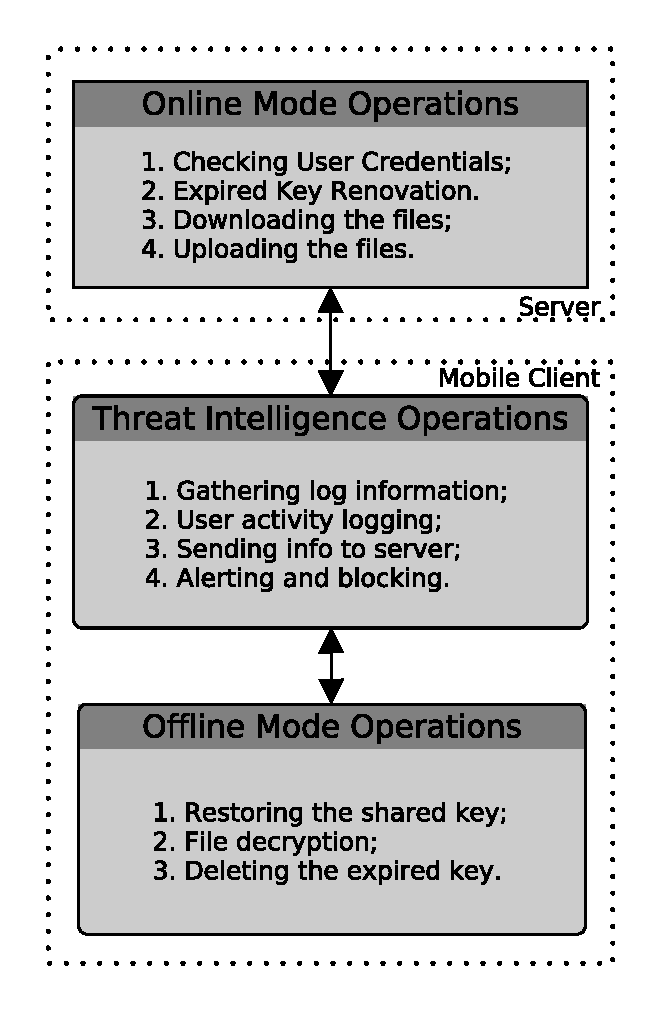
\includegraphics[width=5cm]{../figures/fig01.eps}
		\caption{The core set of functions and protocols of the mobile cloud security infrastructure}
		\label{fig:3_01}
	\end{figure}
	
\end{frame}
% %-=-=-=-=-=-=-=-=-=-=-=-=-=-=-=-=-=-=-=-=-=-=-=-=
% %	FRAME: The Client-side Architecture
% %-=-=-=-=-=-=-=-=-=-=-=-=-=-=-=-=-=-=-=-=-=-=-=-=
% \begin{frame}[c]{The Client-side Architecture}
	
% 	\begin{figure}[h!]
% 		\centering
% 		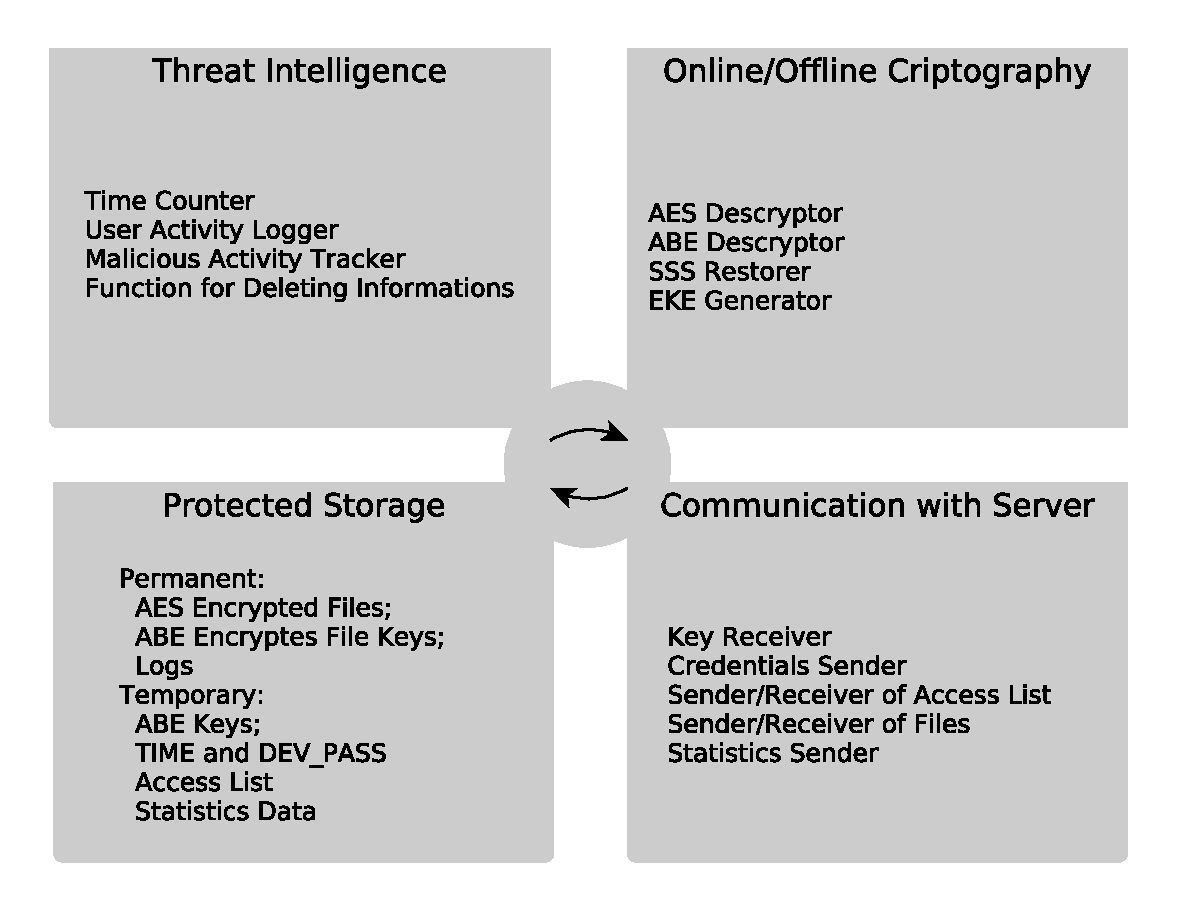
\includegraphics[width=9cm]{../figures/fig02.eps}
% 		\caption{The Client-side Architecture}
% 		\label{fig:3_02}
% 	\end{figure}
	
% \end{frame}
%-=-=-=-=-=-=-=-=-=-=-=-=-=-=-=-=-=-=-=-=-=-=-=-=
%	FRAME: Proposal for offline mobile security
%-=-=-=-=-=-=-=-=-=-=-=-=-=-=-=-=-=-=-=-=-=-=-=-=
\begin{frame}[c]{Proposal for offline mobile security}
	
	\begin{figure}[h!]
		\centering
		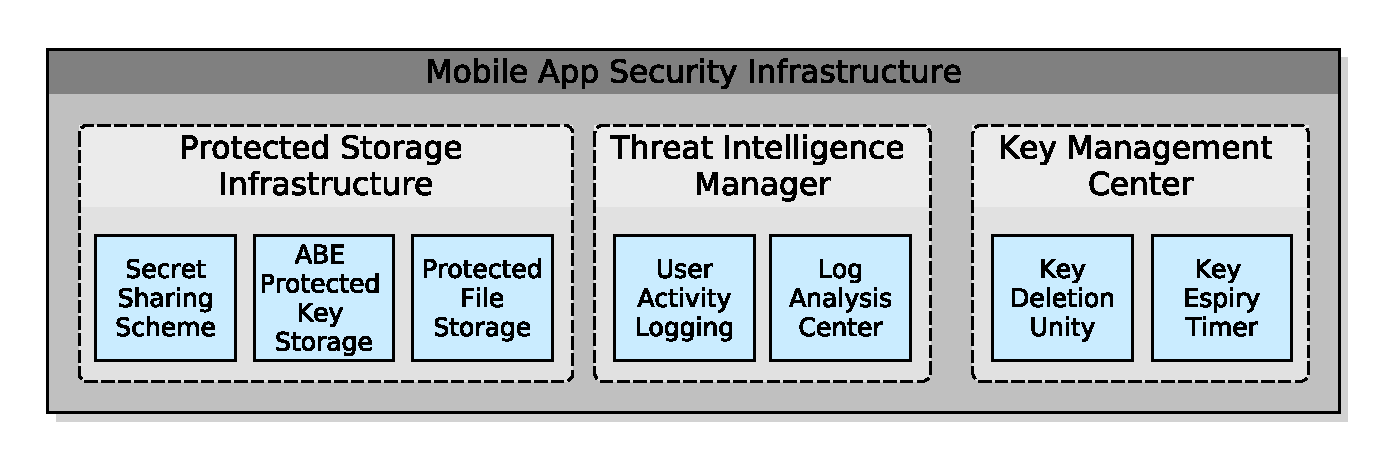
\includegraphics[width=11cm]{../figures/fig03.eps}
		\caption{Proposed Architecture for Offline Mobile Security}
		\label{fig:3_03}
	\end{figure}
	
\end{frame}
%-=-=-=-=-=-=-=-=-=-=-=-=-=-=-=-=-=-=-=-=-=-=-=-=
%	FRAME: Offline Behavioral Analysis
%-=-=-=-=-=-=-=-=-=-=-=-=-=-=-=-=-=-=-=-=-=-=-=-=
\begin{frame}[c]{Offline Behavioral Analysis}
	
	\begin{figure}[h!]
		\centering
		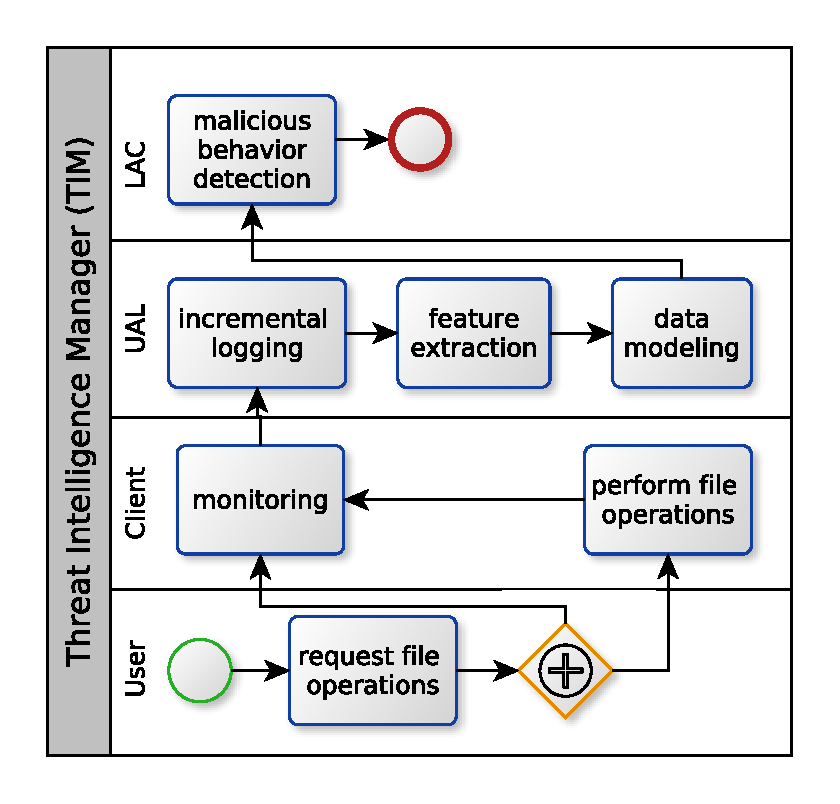
\includegraphics[width=7cm]{../figures/fig06.eps}
		\caption{The Threat Intelligence Manager Workflow}
		\label{fig:3_06}
	\end{figure}
	
\end{frame}
%-=-=-=-=-=-=-=-=-=-=-=-=-=-=-=-=-=-=-=-=-=-=-=-=
%	FRAME: MOS for Threat Intelligence
%-=-=-=-=-=-=-=-=-=-=-=-=-=-=-=-=-=-=-=-=-=-=-=-=
\begin{frame}[c]{MOS for Threat Intelligence}
	
	\begin{itemize}
		\item Largest eigenvalue analysis and MOS (Previously presented);
		\item Applied to user behavior analysis;
		\begin{itemize}
			\item We model file operations as signals (matrices);
			\item We Select features that can highlight malicious behaviors;
			\item We implement and evaluate into mobile devices.
		\end{itemize}
	\end{itemize}
	
\end{frame}
%-=-=-=-=-=-=-=-=-=-=-=-=-=-=-=-=-=-=-=-=-=-=-=-=
%	FRAME: Common threat scenarios
%-=-=-=-=-=-=-=-=-=-=-=-=-=-=-=-=-=-=-=-=-=-=-=-=
\begin{frame}[c]{Common threat scenarios}
	
	\begin{enumerate}
		\item An attacker uses a \textbf{valid password} to perform operations on a \textbf{bulk} of files.;
		\item Usage of \textbf{expired password} to perform unauthorized \textbf{operations};
	\end{enumerate}
	
\end{frame}
%-=-=-=-=-=-=-=-=-=-=-=-=-=-=-=-=-=-=-=-=-=-=-=-=
%	FRAME: Data Modeling for Behavioral Analysis
%-=-=-=-=-=-=-=-=-=-=-=-=-=-=-=-=-=-=-=-=-=-=-=-=
\begin{frame}[c]{Data Modeling for Behavioral Analysis}
	
	Selected features:
	\begin{itemize}
		\item File Access (Time and File System Location);
		\item File Update (Time and File System Location);
		\item File Download (Start Time, End Time and File System Location);
		\item File Upload (Start Time, End Time and File System Location).
	\end{itemize}
	
\end{frame}
%-=-=-=-=-=-=-=-=-=-=-=-=-=-=-=-=-=-=-=-=-=-=-=-=
%	FRAME: Results
%-=-=-=-=-=-=-=-=-=-=-=-=-=-=-=-=-=-=-=-=-=-=-=-=
\begin{frame}[c]{Result: Data Modeling and Eigenvalue Analysis}
		
	\begin{table}
		\tiny
		\label{tab:3_04}
		\centering
		\begin{tabular}{|l|l|l|l|l|l|l|l|}
			\hline \rowcolor{Gray} Device	& \begin{tabular}[x]{@{}l@{}}Log Size\\(MB)\end{tabular}	& \begin{tabular}[x]{@{}l@{}}Window\\(min)\end{tabular}	& \begin{tabular}[x]{@{}l@{}}Modeling\\(ms)\end{tabular}	& \begin{tabular}[x]{@{}l@{}}Avg. Eig.\\(ms)\end{tabular}	& \begin{tabular}[x]{@{}l@{}}Std. Eig.\\(ms)\end{tabular}	& \begin{tabular}[x]{@{}l@{}}Eig. Min.\\(ms)\end{tabular}	& \begin{tabular}[x]{@{}l@{}}Eig. Max.\\(ms)\end{tabular}	\\ \hline
			Galaxy GT-I9300	& 6	& 60	& 107	& 209.52	& 18.58	& 183	& 276	\\ \hline
			Galaxy GT-I9300	& 6	& 40	& 115	& 227.26	& 18.13	& 191	& 289	\\ \hline
			Galaxy GT-I9300	& 6	& 20	& 89	& 268.14	& 21.94	& 229	& 315	\\ \hline
			Galaxy GT-I9300	& 6	& 10	& 90	& 347.42	& 24.11	& 304	& 421	\\ \hline
			Galaxy GT-I9300	& 4.1	& 60	& 20	& 60.90	& 15.19	& 37	& 106	\\ \hline
			Galaxy GT-I9300	& 4.1	& 40	& 20	& 68.72	& 15.71	& 43	& 114	\\ \hline
			Galaxy GT-I9300	& 4.1	& 20	& 34	& 89.04	& 16.78	& 54	& 133	\\ \hline
			Galaxy GT-I9300	& 4.1	& 10	& 21	& 117.24	& 14.36	& 96	& 171	\\ \hline
			Galaxy GT-I9300	& 1.4	& 60	& 10	& 159.82	& 15.82	& 125	& 197	\\ \hline
			Galaxy GT-I9300	& 1.4	& 40	& 10	& 168.06	& 15.90	& 139	& 220	\\ \hline
			Galaxy GT-I9300	& 1.4	& 20	& 11	& 204.4	& 20.46	& 176	& 269	\\ \hline
			Galaxy GT-I9300	& 1.4	& 10	& 13	& 259.00	& 21.34	& 220	& 315	\\ \hline
			Galaxy Tab SM-T800	& 6	& 60	& 7	& 59.30	& 6.55	& 54	& 74	\\ \hline
			Galaxy Tab SM-T800	& 6	& 40	& 8	& 62.56	& 7.05	& 56	& 80	\\ \hline
			Galaxy Tab SM-T800	& 6	& 20	& 10	& 73.28	& 8.59	& 65	& 95	\\ \hline
			Galaxy Tab SM-T800	& 6	& 10	& 8	& 93.48	& 9.13	& 83	& 130	\\ \hline
			Galaxy Tab SM-T800	& 4.1	& 60	& 11	& 18.64	& 4.51	& 16	& 38	\\ \hline
			Galaxy Tab SM-T800	& 4.1	& 40	& 11	& 19.64	& 5.12	& 17	& 38	\\ \hline
			Galaxy Tab SM-T800	& 4.1	& 20	& 12	& 25.12	& 5.55	& 21	& 46	\\ \hline
			Galaxy Tab SM-T800	& 4.1	& 10	& 12	& 32.32	& 7.29	& 27	& 55	\\ \hline
			Galaxy Tab SM-T800	& 1.4	& 60	& 4	& 49.08	& 6.01	& 42	& 62	\\ \hline
			Galaxy Tab SM-T800	& 1.4	& 40	& 5	& 51.42	& 7.36	& 44	& 74	\\ \hline
			Galaxy Tab SM-T800	& 1.4	& 20	& 5	& 51.12	& 7.80	& 54	& 91	\\ \hline
			Galaxy Tab SM-T800	& 1.4	& 10	& 7	& 75.24	& 7.71	& 65	& 90	\\ \hline
		\end{tabular}
	\end{table}
	
\end{frame}
%-=-=-=-=-=-=-=-=-=-=-=-=-=-=-=-=-=-=-=-=-=-=-=-=
%	FRAME: Results
%-=-=-=-=-=-=-=-=-=-=-=-=-=-=-=-=-=-=-=-=-=-=-=-=
\begin{frame}[c]{Result: EDC MOS}
	
	\begin{table}[!t]
		\tiny
		\label{tab:3_05}
		\centering
		\begin{tabular}{|l|l|l|l|l|l|l|l|}
			\hline \rowcolor{Gray} Device	& \begin{tabular}[x]{@{}l@{}}Log Size\\(MB)\end{tabular}	& \begin{tabular}[x]{@{}l@{}}Window\\(min)\end{tabular}	& \begin{tabular}[x]{@{}l@{}}Avg. EDC.\\(ms)\end{tabular}	& \begin{tabular}[x]{@{}l@{}}Std. EDC.\\(ms)\end{tabular}	& \begin{tabular}[x]{@{}l@{}}Min. EDC.\\(ms)\end{tabular}	& \begin{tabular}[x]{@{}l@{}}Max. EDC.\\(ms)\end{tabular}	\\ \hline
			Galaxy GT-I9300	& 6	& 60	& 5.27	& 4.04	& 3	& 20	\\ \hline
			Galaxy GT-I9300	& 6	& 40	& 10.78	& 6.37	& 6	& 34	\\ \hline
			Galaxy GT-I9300	& 6	& 20	& 32.62	& 12.44	& 21	& 88	\\ \hline
			Galaxy GT-I9300	& 6	& 10	& 115.08	& 17.45	& 88	& 158	\\ \hline
			Galaxy GT-I9300	& 4.1	& 60	& 5.68	& 4.18	& 3	& 23	\\ \hline
			Galaxy GT-I9300	& 4.1	& 40	& 10.76	& 5.31	& 7	& 27	\\ \hline
			Galaxy GT-I9300	& 4.1	& 20	& 37.58	& 10.30	& 23	& 61	\\ \hline
			Galaxy GT-I9300	& 4.1	& 10	& 125.98	& 18.56	& 101	& 191	\\ \hline
			Galaxy GT-I9300	& 1.4	& 60	& 4.92	& 3.49	& 3	& 17	\\ \hline
			Galaxy GT-I9300	& 1.4	& 40	& 9.00	& 4.23	& 6	& 25	\\ \hline
			Galaxy GT-I9300	& 1.4	& 20	& 30.14	& 9.21	& 19	& 62	\\ \hline
			Galaxy GT-I9300	& 1.4	& 10	& 100.62	& 15.83	& 69	& 163	\\ \hline
			Galaxy Tab SM-T800	& 6	& 60	& 1.84	& 0.65	& 1	& 3	\\ \hline
			Galaxy Tab SM-T800	& 6	& 40	& 3.26	& 1.24	& 2	& 7	\\ \hline
			Galaxy Tab SM-T800	& 6	& 20	& 10.90	& 2.40	& 9	& 21	\\ \hline
			Galaxy Tab SM-T800	& 6	& 10	& 41.86	& 7.33	& 34	& 60	\\ \hline
			Galaxy Tab SM-T800	& 4.1	& 60	& 1.85	& 0.60	& 1	& 3	\\ \hline
			Galaxy Tab SM-T800	& 4.1	& 40	& 3.62	& 1.10	& 2	& 8	\\ \hline
			Galaxy Tab SM-T800	& 4.1	& 20	& 12.04	& 2.79	& 9	& 22	\\ \hline
			Galaxy Tab SM-T800	& 4.1	& 10	& 40.16	& 6.48	& 35	& 60	\\ \hline
			Galaxy Tab SM-T800	& 1.4	& 60	& 1.98	& 0.89	& 1	& 6	\\ \hline
			Galaxy Tab SM-T800	& 1.4	& 40	& 3.30	& 1.16	& 2	& 7	\\ \hline
			Galaxy Tab SM-T800	& 1.4	& 20	& 10.48	& 2.90	& 8	& 21	\\ \hline
			Galaxy Tab SM-T800	& 1.4	& 10	& 34.52	& 4.08	& 30	& 45	\\ \hline
		\end{tabular}
	\end{table}
	
\end{frame}
%-=-=-=-=-=-=-=-=-=-=-=-=-=-=-=-=-=-=-=-=-=-=-=-=
%	FRAME: Results
%-=-=-=-=-=-=-=-=-=-=-=-=-=-=-=-=-=-=-=-=-=-=-=-=
\begin{frame}[c]{Results}
	
	\begin{itemize}
		\item The \textbf{lower window} size leads to the \textbf{larger eigenvalue analysis time};
		\item The largest eigenvalue analysis time: 421 milliseconds with average of 347.42 milliseconds;
		\item The \textbf{MOS} processing time \textbf{increases} with the \textbf{window size decreasing};
		\item The longest MOS processing time: lower than 200 milliseconds;
		\item This results represent an \textbf{acceptable processing time} for \textbf{anomaly detection in mobile clients}.
	\end{itemize}
	
\end{frame}


%-=-=-=-=-=-=-=-=-=-=-=-=-=-=-=-=-=-=-=-=-=-=-=-=
%
%	SECTION: Tensor-based Discriminative Sensing for Fraud Detection
%
%-=-=-=-=-=-=-=-=-=-=-=-=-=-=-=-=-=-=-=-=-=-=-=-=
\section{Tensor-based Discriminative Sensing for Fraud Detection}
%-=-=-=-=-=-=-=-=-=-=-=-=-=-=-=-=-=-=-=-=-=-=-=-=
%	FRAME: Introduction
%-=-=-=-=-=-=-=-=-=-=-=-=-=-=-=-=-=-=-=-=-=-=-=-=
\begin{frame}[c]{Introduction}
	\begin{itemize}
		\item A \textbf{key challenge} to use sparse coding and dictionary learning for \textbf{classification} is how to find \textbf{proper dictionaries and coefficients};
		\item The data and its dictionary can be \textbf{multidimensional};
		\item \textbf{Tensor decompositions} can be useful to extract \textbf{hidden patterns} and structure in \textbf{multidimensional} data analytics problems;
		\item The \textbf{fundamental issue} with the \textbf{imbalanced learning} problem is the ability of imbalanced data to \textbf{compromise the performance of algorithms} \cite{he2009learning};
	\end{itemize}
\end{frame}
%-=-=-=-=-=-=-=-=-=-=-=-=-=-=-=-=-=-=-=-=-=-=-=-=
%	FRAME: Introduction
%-=-=-=-=-=-=-=-=-=-=-=-=-=-=-=-=-=-=-=-=-=-=-=-=
\begin{frame}[c]{Introduction}
	\begin{itemize}
		\item We propose a tensor-based sparse representation and dictionary learning technique to analyze mobile money transactions in order to identify frauds.
	% 	\item Tensor-based DL for learning fraudulent and legitimate data separately
	% 	\item Apply the learned dictionaries to reconstruct a test signal and classify it as fraud or legitimate.
	\end{itemize}
\end{frame}
%-=-=-=-=-=-=-=-=-=-=-=-=-=-=-=-=-=-=-=-=-=-=-=-=
%	FRAME: Motivation: Tensor-based Dictionary Recovery
%-=-=-=-=-=-=-=-=-=-=-=-=-=-=-=-=-=-=-=-=-=-=-=-=
\begin{frame}[c]{Motivation: Tensor-based Dictionary Recovery}
	\begin{itemize}
		\item Tensor-based algorithms for recovering of a known separable dictionary outperform existing schemes when dealing with growing multidimensional datasets.
	\end{itemize}
\end{frame}
%-=-=-=-=-=-=-=-=-=-=-=-=-=-=-=-=-=-=-=-=-=-=-=-=
%	FRAME: Motivation: Tensor-based Dictionary Recovery
%-=-=-=-=-=-=-=-=-=-=-=-=-=-=-=-=-=-=-=-=-=-=-=-=
\begin{frame}[c]{Motivation: Tensor-based Dictionary Recovery}

	We consider a \textbf{generic sparse recovery problem}
	\begin{equation}\label{eq:4_eq01}
		\textbf{X} = \textbf{A} \cdot \textbf{S} + \textbf{W},
	\end{equation}
	where $\textbf{X} \in \mathbb{C}^{M \times T}$ represents $T$ consecutive observations from $M$ features, $\textbf{A} \in \mathbb{C}^{M \times N}$ is the overcomplete dictionary where $N \ll T$, $\textbf{S} \in \mathbb{C}^{N \times T}$ represents the sparse coefficient matrix, $\textbf{W} \in \mathbb{C}^{M \times T}$ is the additive noise, and $M < N < T$.

\end{frame}
%-=-=-=-=-=-=-=-=-=-=-=-=-=-=-=-=-=-=-=-=-=-=-=-=
%	FRAME: Motivation: Tensor-based Dictionary Recovery
%-=-=-=-=-=-=-=-=-=-=-=-=-=-=-=-=-=-=-=-=-=-=-=-=
\begin{frame}[c]{Motivation: Tensor-based Dictionary Recovery}

	Based on Roemer \emph{et al} \cite{roemer2014tensor}, we consider a sparse recovery problem for a \textbf{separable 2-D dictionary} that we can write as
	\begin{equation}\label{eq:4_eq02}
		\textbf{X} = (\textbf{A}^{(1)} \otimes \textbf{A}^{(2)}) \cdot \textbf{S} + \textbf{W},
	\end{equation}
	where $\textbf{A} = (\textbf{A}^{(1)} \otimes \textbf{A}^{(2)})$, $\textbf{A}^{(1)} \in \mathbb{C}^{M_1 \times N_1}$, $\textbf{A}^{(2)} \in \mathbb{C}^{M_2 \times N_2}$, $M = M_1 \times M_2$, and $N = N_1 \times N_2$.

\end{frame}
%-=-=-=-=-=-=-=-=-=-=-=-=-=-=-=-=-=-=-=-=-=-=-=-=
%	FRAME: Motivation: Tensor-based Dictionary Recovery
%-=-=-=-=-=-=-=-=-=-=-=-=-=-=-=-=-=-=-=-=-=-=-=-=
\begin{frame}[c]{Motivation: Tensor-based Dictionary Recovery}

	We \textbf{generate two random dictionaries} $\textbf{A}^{(1)}$ and $\textbf{A}^{(2)}$ from an i.i.d. zero mean Gaussian random process, and calculate the known dictionary $\textbf{A}$
	\begin{equation}\label{eq:4_eq03}
		\textbf{A} = (\textbf{A}^{(1)} \otimes \textbf{A}^{(2)}).
	\end{equation}

\end{frame}
%-=-=-=-=-=-=-=-=-=-=-=-=-=-=-=-=-=-=-=-=-=-=-=-=
%	FRAME: Motivation: Tensor-based Dictionary Recovery
%-=-=-=-=-=-=-=-=-=-=-=-=-=-=-=-=-=-=-=-=-=-=-=-=
\begin{frame}[c]{Motivation: Tensor-based Dictionary Recovery}

	Generate a synthetic data set $\textbf{X}$ from $\textbf{A}$

	Estimate the initial $\hat{\textbf{A}}$ and make the dictionary separable decomposing the approximation of $\hat{\textbf{A}}$ and generating $\hat{\textbf{A}}^{(1)}$ and $\hat{\textbf{A}}^{(2)}$
	\begin{equation}\label{eq:4_eq04}
		\hat{\textbf{A}} = (\hat{\textbf{A}}^{(1)} \otimes \hat{\textbf{A}}^{(2)}),
	\end{equation}
	and use it for DL recovery experiments using MOD, K-SVD, RLS-DLA, T-MOD and K-HOSVD. 

\end{frame}
%-=-=-=-=-=-=-=-=-=-=-=-=-=-=-=-=-=-=-=-=-=-=-=-=
%	FRAME: Motivation: Tensor-based Dictionary Recovery
%-=-=-=-=-=-=-=-=-=-=-=-=-=-=-=-=-=-=-=-=-=-=-=-=
\begin{frame}[c]{Motivation: Tensor-based Dictionary Recovery}
	\begin{figure}[!htb]
		\centering 
		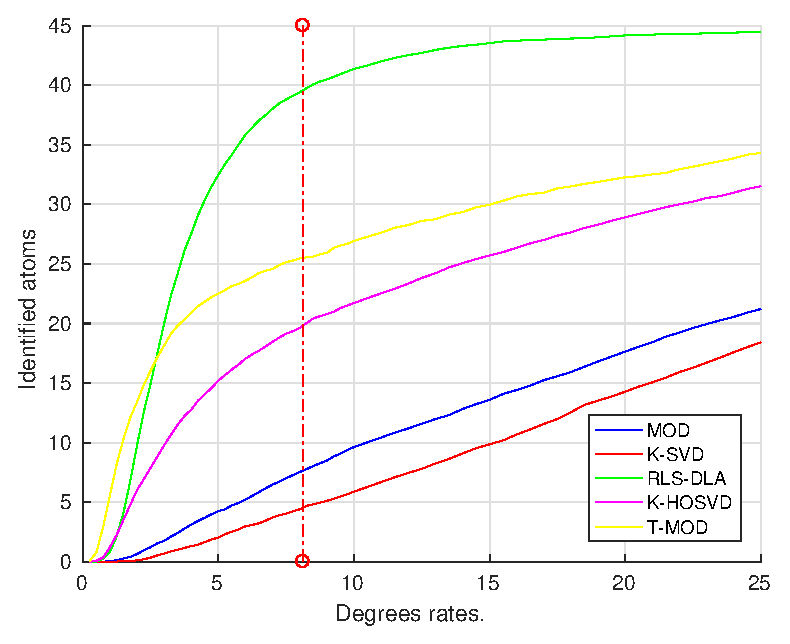
\includegraphics[width=10cm]{../figures/ch4/s=5_snr=20_L=2000_noIt=100_N=20_K=50.eps}
		\caption{Cumulative atom identification per degree rates. $T=2000$, $M=20$, $N=50$}
		\label{fig:fig1}
	\end{figure}
\end{frame}
%-=-=-=-=-=-=-=-=-=-=-=-=-=-=-=-=-=-=-=-=-=-=-=-=
%	FRAME: Motivation: Tensor-based Dictionary Recovery
%-=-=-=-=-=-=-=-=-=-=-=-=-=-=-=-=-=-=-=-=-=-=-=-=
\begin{frame}[c]{Motivation: Tensor-based Dictionary Recovery}
	\begin{figure}[!htb]
		\centering 
		\includegraphics[width=10cm]{../figures/ch4/5_20_2000_24000_100.eps}
		\caption{Cumulative atom identification per degree rates. $T=2000$, $M=80$, $N=300$}
		\label{fig:fig2}
	\end{figure}
\end{frame}
%-=-=-=-=-=-=-=-=-=-=-=-=-=-=-=-=-=-=-=-=-=-=-=-=
%	FRAME: Related Works
%-=-=-=-=-=-=-=-=-=-=-=-=-=-=-=-=-=-=-=-=-=-=-=-=
\begin{frame}[c]{Related Works}

	\begin{itemize}
		\item Wright \emph{et al} \cite{wright2009robust} have proposed a face \textbf{recognition method} that uses training face images as dictionaries and an $l_1$ sparse optimization method in the classification stage. The authors show that the recognition task can be \textbf{successfully} accomplished even using \textbf{random features};
		\item Roemer \emph{et al} \cite{roemer2014tensor} have proposed a \textbf{tensor-based multidimensional extensions for MOD and K-SVD algorithms} and show their improved performances numerically, for the dictionary reconstruction problem;
		\item To the best of our knowledge \textbf{there is no similar model} applied to \textbf{fraud detection}.
	\end{itemize}

\end{frame}
%-=-=-=-=-=-=-=-=-=-=-=-=-=-=-=-=-=-=-=-=-=-=-=-=
%	FRAME: Data Model
%-=-=-=-=-=-=-=-=-=-=-=-=-=-=-=-=-=-=-=-=-=-=-=-=
\begin{frame}[c]{Data Model}

	\begin{itemize}
		\item We adopt a synthetic financial datasets for fraud detection generated by PaySim;
		\begin{itemize}
			\item 9 features (variables);
			\item 2.770.408 transactions(observations);
			\item labels to classify fraudulent or legitimate transactions;
			\item 2.762.195 of normal transactions.
			\item 8.213 fraudulent transactions(0,30 \%);
		\end{itemize}
	\end{itemize}

	Training data as $\textbf{X}_r$,  test data as $\textbf{X}_e$. 

	Normal train data is $\textbf{X}_r^o$ and fraud train data is $\textbf{X}_r^f$. 

	The same notation is applied to qualify $\textbf{A}$ and $\textbf{S}$.

\end{frame}
%-=-=-=-=-=-=-=-=-=-=-=-=-=-=-=-=-=-=-=-=-=-=-=-=
%	FRAME: Tensor-based Sparse Representation Classification
%-=-=-=-=-=-=-=-=-=-=-=-=-=-=-=-=-=-=-=-=-=-=-=-=
\begin{frame}[c]{Tensor-based Sparse Representation Classification}

	\begin{itemize}
		\item \textbf{Split} the training data into \textbf{fraud and normal} ($\textbf{X}_r^f$ and $\textbf{X}_r^o$);
		\item \textbf{Estimate} the initial dictionaries $\hat{\textbf{A}}_r^f$ and $\hat{\textbf{A}}_r^o$;
		\item Apply the \textbf{dictionaries} and the \textbf{data matrices} to the selected \textbf{DL algorithm} for learning the \textbf{best dictionaries} $\hat{\textbf{A}}_r^f$ and $\hat{\textbf{A}}_r^o$;
		\item Process each transaction of $\textbf{X}_e$, denoted as $\textbf{x}_t$, to generate  $\hat{\textbf{s}}_t^f$ and $\hat{\textbf{s}}_t^o$;
		\item Compute signal reconstruction for each test transaction $t$
			\begin{equation}\label{eq:4_eq041}
				\hat{\textbf{x}}_t^f = \hat{\textbf{A}}_r^f \cdot \hat{\textbf{s}}_t^f
			\end{equation}
			\begin{equation}\label{eq:4_eq042}
				\hat{\textbf{x}}_e^o = \hat{\textbf{A}}_r^o \cdot \hat{\textbf{s}}_e^o
			\end{equation}
		\item Compare $\hat{\textbf{x}}_t^f$ and $\hat{\textbf{x}}_t^o$ to $\textbf{x}_t$ to classify the transaction as fraud or normal according to the minimum reconstruction error.
	\end{itemize}

\end{frame}
%-=-=-=-=-=-=-=-=-=-=-=-=-=-=-=-=-=-=-=-=-=-=-=-=
%	FRAME: Experiments
%-=-=-=-=-=-=-=-=-=-=-=-=-=-=-=-=-=-=-=-=-=-=-=-=
\begin{frame}[c]{Experiments}

	\begin{itemize}
		\item We propose to evaluate the \textbf{K-HOSVD} to analyze how a tensor-based DL algorithm can highlight the \textbf{discriminative structure for fraud detection};
		\item We compare the proposed approach against the \textbf{Support Vector Machines (SVM) Logistic Regression (LR) using PCA data};
		\item We adopt the area under the Receiver Operating Characteristic (\textbf{ROC}) curve and the area under the Precision-Recall (\textbf{PR}) curve.
	\end{itemize}

\end{frame}
%-=-=-=-=-=-=-=-=-=-=-=-=-=-=-=-=-=-=-=-=-=-=-=-=
%	FRAME: Results
%-=-=-=-=-=-=-=-=-=-=-=-=-=-=-=-=-=-=-=-=-=-=-=-=
\begin{frame}[c]{Results}

	\begin{table}[h!]
	  \centering
	  \scriptsize
	  \caption{Results for fraud detection from mobile money transactions} 
	  \label{tab:4_tab1}
	  \begin{tabular}{ c c c c c }
		\toprule
		\multirow{2}{*}{\textbf{Classifier}}   &\multicolumn{2}{c}{\textbf{undersample/undersample}} &\multicolumn{2}{c}{\textbf{undersample/complete}}\\ 
				\hhline{~----}
				&\textbf{ROC-AUC} &\textbf{PR-AUC} &\textbf{ROC-AUC} &\textbf{PR-AUC}\\
		\midrule
		SVM &0.5039 &0.7493 &0.8496 &\color{red}0.8497 \\
		LR with PCA &\color{red}0.9767 &\color{red}0.9793 &0.5633 &0.0051 \\
		K-HOSVD ($K=3$, $N=40$) &0.8622 &0.8917 &\color{red}0.8652 &0.4578 \\
	    \bottomrule
	  \end{tabular}
	\end{table}

\end{frame}
%-=-=-=-=-=-=-=-=-=-=-=-=-=-=-=-=-=-=-=-=-=-=-=-=
%	FRAME: Results
%-=-=-=-=-=-=-=-=-=-=-=-=-=-=-=-=-=-=-=-=-=-=-=-=
\begin{frame}[c]{Results}

	\begin{itemize}
		\item \textbf{SVM} presents the \textbf{best PR-AUC for generalization}, but its \textbf{PR-AUC} was the \textbf{worst} for training and testing with \textbf{undersampled} data;
		\item \textbf{LR with PCA} data presents the \textbf{best} results for training and testing with \textbf{undersampled} data, but the \textbf{complete} testing data presents a \textbf{very low PR-AUC};
		\item \textbf{K-HOSVD} presents \textbf{higher PR-AUC than SVM} for \textbf{undersampled} data, but its results are \textbf{worst than LR with PCA} for the same scenario;
		\item \textbf{K-HOSVD} presents \textbf{better PR-AUC than LR with PCA} and the \textbf{best ROC-AUC} for training the undersampled data and test with \textbf{complete} data.
	\end{itemize}

\end{frame}
%-=-=-=-=-=-=-=-=-=-=-=-=-=-=-=-=-=-=-=-=-=-=-=-=
%	FRAME: Results
%-=-=-=-=-=-=-=-=-=-=-=-=-=-=-=-=-=-=-=-=-=-=-=-=
\begin{frame}[c]{Results}

	Our \textbf{approach} presents \textbf{average results} if compared to two well known and highly adopted \textbf{classifier algorithms for fraud detection} from mobile money transactions.

\end{frame}


%-=-=-=-=-=-=-=-=-=-=-=-=-=-=-=-=-=-=-=-=-=-=-=-=
%
%	SECTION: Conclusion and Future Work
%
%-=-=-=-=-=-=-=-=-=-=-=-=-=-=-=-=-=-=-=-=-=-=-=-=
\section{Conclusion and Future Work}
%-=-=-=-=-=-=-=-=-=-=-=-=-=-=-=-=-=-=-=-=-=-=-=-=
%	FRAME: Conclusion
%-=-=-=-=-=-=-=-=-=-=-=-=-=-=-=-=-=-=-=-=-=-=-=-=
\begin{frame}[c]{Conclusion}

	\begin{itemize}
		\item \textbf{Synflood, fraggle and port scan attacks can be detected accurately and with great detail in an automatic and blind fashion}, applying signal processing concepts for traffic modeling and through approaches based on MOS and eigen similarity analysis;
		\item This thesis presented a proposal to address the \textbf{offline mobile security} problem through malicious behavior analysis. The solution has \textbf{positive results in terms of performance};
		\item A \textbf{tensor-based DL} approach can be used for \textbf{fraud detection} from mobile money transactions, with \textbf{average results}.
	\end{itemize}

\end{frame}
%-=-=-=-=-=-=-=-=-=-=-=-=-=-=-=-=-=-=-=-=-=-=-=-=
%	FRAME: Contributions
%-=-=-=-=-=-=-=-=-=-=-=-=-=-=-=-=-=-=-=-=-=-=-=-=
% \begin{frame}[c]{Contributions}
% 	\begin{enumerate}
% 		\item We proposed an approach based on eigen similarity analysis for extracting detailed information about accurate time and network ports under network attack, and evaluated the accuracy and performance of the proposed framework applied to an experimental scenario and to the DARPA 1998 dataset;
% 		\item We discussed the computational complexity of the proposed framework and evaluated the required processing time for tested scenarios;
% 		\item We proposed an architecture and techniques for offline behavioral analysis of a corporate mobile client security architecture;
% 		\item We discussed the processing time of the proposed framework for mobile devices.
% 	\end{enumerate}
% \end{frame}
%-=-=-=-=-=-=-=-=-=-=-=-=-=-=-=-=-=-=-=-=-=-=-=-=
%	FRAME: Contributions
%-=-=-=-=-=-=-=-=-=-=-=-=-=-=-=-=-=-=-=-=-=-=-=-=
\begin{frame}[c]{Contributions}
	\begin{enumerate}
		% \item We proposed a tensor-based dictionary learning approach for fraud detection in mobile payment transactions;
		\item We published the following papers reporting our results:
		\begin{enumerate}
			\item T. P. B. Vieira, D. F. Ten\'orio, J. P. C. L. da Costa, E. P. de Freitas, G. Del Galdo, and R. T. de Sousa J\'unior, \textit{Model Order Selection and Eigen Similarity based Framework for Detection and Identication of Network Attacks}. Journal of Networking and Computer Applications (JNCA), Vol 90, Jul 2017, Pages 26–41.
			\item T. Galibus, T. P. B. Vieira, E. P. de Freitas, R. Albuquerque, J. P. C. L. da Costa, R. T. de Sousa Jr, V. Krasnoproshin, A. Zaleski, H. Vissia, and G. del Galdo, \textit{Offline Mode for Corporate Mobile Client Security Architecture}. Mobile Networks and Applications, Springer, Mar 2017, Pages 1-17.
		\end{enumerate}
	\end{enumerate}
\end{frame}
%-=-=-=-=-=-=-=-=-=-=-=-=-=-=-=-=-=-=-=-=-=-=-=-=
%	FRAME: Future Work
%-=-=-=-=-=-=-=-=-=-=-=-=-=-=-=-=-=-=-=-=-=-=-=-=
\begin{frame}[c]{Future Work}
	\begin{enumerate}
		\item To adopt one dictionary with basis vectors that represent legitimate and fraudulent data, as a \textbf{concatenation or as a kronecker product};
		\item To adopt \textbf{discriminative functions} for T-MOD and K-HOSVD, such as the Fisher discrimination criterion;
		\item To extend the evaluation for other \textbf{DL algorithms}.
		% \item Improvements for obtaining better false positive rates, as well as for make the proposed framework able to identify sparse probe attacks or subtle behaviors, such as exfiltration or covert communication, considering the evaluation of a flow-based analysis and novel datasets;
		% \item Distributed or parallel processing can also be evaluated to analyze the scalability and processing capacity for monitoring high throughput network traffic;
		% \item Evaluate the application of the proposed approach to different attack types and domains, considering cases that are aware to behavioral analysis;
		% \item Explore enhancements in the analytics methods as well as to extended the approach to be used by mobile devices with even more severe resources constraints;
	\end{enumerate}
\end{frame}

%-=-=-=-=-=-=-=-=-=-=-=-=-=-=-=-=-=-=-=-=-=-=-=-=
%	FRAME: Bibliography
%-=-=-=-=-=-=-=-=-=-=-=-=-=-=-=-=-=-=-=-=-=-=-=-=
\begin{frame}[plain, allowframebreaks]{Bibliography}
	\setbeamertemplate{bibliography item}[text]
	\printbibliography
\end{frame}

\end{document}